%This is a very basic  BE PROJECT PRELIMINARY template.

%############################################# 
%#########Author :  PROJECT###########
%#########COMPUTER ENGINEERING############


\documentclass[twoside,a4paper,12pt]{book}
\usepackage{fancyhdr}
\usepackage{amsmath}
\usepackage{xpatch}
%\usepackage{ltxfront}
\usepackage{titlesec}
\usepackage{titletoc}
%\usepackage{afterpage}
%\usepackage{ltxgrid}
\usepackage{booktabs}
%\hoffset = 8.9436619718309859154929577464789pt
%\voffset = 13.028169014084507042253521126761pt
  

\fancypagestyle{plain}{
  \fancyhf{}
  \fancyhead[LE]{Avoiding Road Traffic Congestion using PSO}
  \fancyhead[RO]{\thechapter}
  \renewcommand{\headrulewidth}{1pt}
  \fancyfoot[LE]{PESMCOE, Department of Computer Engineering 2016-17}
  \fancyfoot[RE]{\thepage}
  \renewcommand{\footrulewidth}{1pt}  
}

\fancypagestyle{special}{
  \fancyhf{}
  \renewcommand{\headrulewidth}{0pt}
  \renewcommand{\footrulewidth}{1pt}
  \fancyfoot[C]{\thepage}
}

\fancypagestyle{clear}{
  \fancyhf{}
  \renewcommand{\headrulewidth}{0pt}
  \renewcommand{\footrulewidth}{0pt}
}

\usepackage[]{hyperref}
\usepackage{tikz}
%\usetikzlibrary{arrows,shapes,snakes,automata,backgrounds,petri}

\usepackage{tabularx}

\usepackage[nottoc,notlot,notlof,numbib]{tocbibind}
\usepackage[titletoc]{appendix}

\renewcommand{\appendixname}{Annexure}
\usepackage{titletoc}
\renewcommand{\bibname}{References}
%\renewcommand{\chaptername}{References}
%\renewcommand\bibname{References}
\setcounter{secnumdepth}{5}
%\setcounter{page}{-1}
\usepackage{float}
%\usepackage{subcaption}
%\usepackage{multirow}

%\usepackage[ruled,vlined]{algorithm2e}

\begin{document}

\pagestyle{empty}
%=======================================================================

% Report Front Page

\pagenumbering{gobble}
\setlength{\parindent}{0mm}
\begin{center}

{\bfseries A  PROJECT REPORT ON \\}
 \vspace*{2\baselineskip}
{\bfseries \fontsize{16}{16} \selectfont AVOIDING ROAD TRAFFIC CONGESTION USING PARTICLE SWARM OPTIMISATION \\ \vspace*{2\baselineskip}}
{\fontsize{12}{12} \selectfont SUBMITTED TO THE SAVITRIBAI PHULE PUNE UNIVERSITY , PUNE
IN THE PARTIAL FULFILLMENT OF THE REQUIREMENTS 
FOR THE AWARD OF THE DEGREE
\\

\vspace*{2\baselineskip}}
{\bfseries \fontsize{14}{12} \selectfont BACHELOR OF ENGINEERING\\
 (Computer Engineering) \\
\vspace*{1\baselineskip}} 
{\bfseries \fontsize{14}{12} \selectfont BY \\ 
\vspace*{1\baselineskip}} 
\hspace*{15mm}Adil Hussain \hfill Exam No: B120314204\hspace*{15mm} \\
\hspace*{15mm}Mohammad Moheed Inamdar \hfill Exam No: B120314249\hspace*{15mm}  \\
\hspace*{15mm}Ajay Singh Rajpurohit \hfill Exam No: B120314310\hspace*{15mm} \\
\hspace*{15mm}Utkarsh Alone \hfill Exam No: B120314207\hspace*{15mm} \\
\vspace*{2\baselineskip}
{\bfseries \fontsize{14}{12} \selectfont Under the guidance of : \\}
Prof. Mrs. Deepti Nirwal\\

\includegraphics[height=1.5in, width=2.5in,keepaspectratio]{collegelogo.png}\\[6mm]
\fontsize{14}{5pt}\selectfont
\textbf{DEPARTMENT OF COMPUTER ENGINEERING\vspace*{1\baselineskip}
 PES MODERN COLLEGE OF ENGINEERING}\\

\fontsize{12}{12pt}\selectfont
SHIVAJINAGAR,PUNE 411005 \\[5mm]


\fontsize{14}{12pt}\selectfont
\textbf{SAVITRIBAI PHULE PUNE UNIVERSITY, PUNE}\\
\textbf{2017 - 18}     
\end{center}

%=======================================================================

% Certificate Page



\newpage

\begin{figure}[ht]
\centering

\includegraphics[height=1.6in, width=2.5in,keepaspectratio]{collegelogo.png}\\[6mm]
\end{figure}


{\bfseries \fontsize{16}{12} \selectfont \centerline{CERTIFICATE} 
\vspace*{2\baselineskip}} 

\centerline{This is to certify that the Project Entitled}
\vspace*{.5\baselineskip} 


{\bfseries \fontsize{16}{16} \selectfont \centering AVOIDING ROAD TRAFFIC CONGESTION USING PARTICLE SWARM OPTIMIZATION
\vspace*{0.5\baselineskip}}

\centerline{Submitted by}
\vspace*{0.5\baselineskip} 
\hspace*{15mm}Adil Hussain \hfill Exam No: B120314204\hspace*{15mm} \\
\hspace*{15mm}Mohammad Moheed Inamdar \hfill Exam No: B120314249\hspace*{15mm}  \\
\hspace*{15mm}Ajay Singh Rajpurohit \hfill Exam No: B120314310\hspace*{15mm} \\
\hspace*{15mm}Utkarsh Alone \hfill Exam No: B120314207\hspace*{15mm} \\
\vspace*{0.5\baselineskip}

is a bonafide work carried out by them under the supervision of Prof. Mrs. Deepti Nirwal and it is approved for the partial fulfillment of the requirement of Savtribai Phule Pune university, Pune for the award of the degree of Bachelor of Engineering (Computer Engineering).\\
\vspace*{1\baselineskip}
 
\bgroup
\def\arraystretch{0.7}
\vspace*{0.5\baselineskip}
\begin{tabular}{c c c}
Prof. Mrs. Deepti Nirwal &  \hspace*{2mm} Prof. Dr. Mrs. S. A. ITKAR & \\									
Guide   &  \hspace*{2mm} Head \\
Department of Computer Engineering  & \hspace*{5mm} Department of Computer Engineering  & \\
\end{tabular}
%}
\vspace*{0.5\baselineskip} 
\begin{center}
%\fontsize{12}{18}\selectfont 
{


}
\end{center}
\vspace*{4\baselineskip}
\begin{tabular}{c c c}
\hspace*{6mm}Signature of Internal Examiner&  \hspace*{18mm} Signature of External Examiner & \\
\end{tabular}



%=======================================================================

% Approval Sheet, wtf is this?

\newpage

\begin{center}
\textbf{PROJECT APPROVAL SHEET}
\end{center}
\begin{center}
 A Project Report Titled as
 \end{center}
\begin{center}
\vspace*{1\baselineskip} 
{\bfseries \fontsize{16}{16} \selectfont \centering AVOIDING ROAD TRAFFIC CONGESTION USING PARTICLE SWARM OPTIMIZATION
\vspace*{0.5\baselineskip}}
\end{center}
\begin{center}
is successfully completed by 
\end{center}
\hspace*{15mm}Adil Hussain \hfill Exam No: B120314204\hspace*{15mm} \\
\hspace*{15mm}Mohammad Moheed Inamdar \hfill Exam No: B120314249\hspace*{15mm}  \\
\hspace*{15mm}Ajay Singh Rajpurohit \hfill Exam No: B120314310\hspace*{15mm} \\
\hspace*{15mm}Utkarsh Alone \hfill Exam No: B120314207\hspace*{15mm} \\
\begin{center}
 at
 \end{center} 
 \begin{center}
 DEPARTMENT OF COMPUTER ENGINEERING
 \end{center}
 \begin{center}
 PES MODERN COLLEGE OF ENGINEERING
 \end{center}
 \begin{center}
 SAVITRIBAI PHULE PUNE UNIVERSITY,PUNE
 \end{center}
 
 \begin{center}
 ACADEMIC YEAR 2017-2018
 \end{center}
 
 \vspace*{7\baselineskip}}
 \begin{tabular}{c c }
Prof. Mrs. Deepti Nirwal &  \hspace*{2mm} Prof. Dr. Mrs. S. A. ITKAR\\									
Guide   &  \hspace*{2mm} Head \\
Department of Computer Engineering  & \hspace*{5mm} Department of Computer Engineering  \\
\end{tabular}

\newpage


%=======================================================================

%classic formatting



\begin{center}
\vspace*{0.4\textwidth}
\emph{This page has been intentionally left empty}    
\end{center}


%========================================================================
%Acknowledgment

{  \newpage {\bfseries \fontsize{20}{12} \selectfont \centerline{Acknowledgement} 
\vspace*{2\baselineskip}} \setlength{\parindent}{11mm} }
{ \setlength{\parindent}{0mm} }
 \pagestyle{special} 
\pagenumbering{roman}
\normalsize
It gives us pleasure in presenting the project report on \textbf{'Avoiding Road Traffic Congestion using Particle Swarm Optimization'}.\\

Firstly, we would like to express our indebtedness appreciation to our guide \textbf{Prof. Mrs. Deepti Nirwal}. Her constant guidance and advice played very important role in successful completion of the project. She always gave us her suggestions, that were crucial in making this report as flawless as possible.\\

We would like to express our gratitude towards \textbf{Prof. Dr. Mrs. S. A. Itkar}  Head of Computer Engineering Department, PES Modern College of Engineering for her kind co-operation and encouragement which helped us during the completion of this report.\\

Also we wish to thank our Principal, \textbf{Prof. Dr. Mrs. K. R. Joshi} and all faculty members for their whole hearted co-operation for completion of this report. We also thank our laboratory assistants for their valuable help in laboratory. \\

Last but not the least, the backbone of our success and confidence lies solely on blessings of dear parents and lovely friends.

\begin{flushright}
Name1\\
Name2\\
Name3\\
Name4\\
\end{flushright}


%=======================================================================

% Abstract is here!!!!

{  \newpage {\bfseries \fontsize{14}{12} \selectfont \centerline{Abstract} 
\vspace*{2\baselineskip}} \setlength{\parindent}{11mm} }
{ \setlength{\parindent}{0mm} }

\noindent
The current traffic control systems work with setting default times for each direction on the crossroads. The traffic style might be the classic one directional, or adjoint-left or two-directional flow, depending on when the signal was installed. If the timings on the signal need to be changed then, one must call for some traffic signal authority to visit the site and manually change the timings.

To allow for changing traffic signal timings without a manual visit, and to allow greater control over signal timings ; Area Traffic Control Systems (ATCS) were introduced. The first ATCS was formulated by Lo (1999) in his paper about handling imminent traffic using the Hydrodynamic Model of Traffic Flow. Systems were henceforth created to predict imminent traffic and work on these numbers to change the Traffic Signal Timings.

Modern ATCS allow the controllers to apply custom traffic control sequences like all-amber (all yellow lights) or all-red (traffic halt) or even manual traffic redirection (setting green for a route, and red for all other directions). Such systems use a central control "master" that is capable of sending commands to each "slave" traffic signal. 






%Traffic management is a tedious task riddled with a lot of uncertainty of buildup and flow changes. The largest issue regarding Traffic Management is its unpredictability of changes. This Project aims to tackle this issue with the use of incremental changes that counteract signs of Traffic buildup. The idea is to detect changes in the traffic density (from cycle to cycle) and slowly increase/decrease signal timings for the growing/shrinking route density or overall.
%This allows us to do 2 things at once, viz.\\
%\\1. Prepare and provide proportional timings to each road of the signal and
%\\2. Dynamically increase/decrease the overall signal cycle time based on density growth/reduction.
%\\ \\ Our system is ideal for use in a Smart City environment or any environment that provides GSM internet or mobile data abilities near the roads

%=======================================================================

%Keywords


{  \newpage {\bfseries \fontsize{14}{12} \selectfont \centerline{Keywords} 
\vspace*{2\baselineskip}} \setlength{\parindent}{11mm} }
{ \setlength{\parindent}{0mm} }

\textbf{\emph{Distributed  Artificial Intelligence, Intelligent agents, Swarm Intelligence}}






%=======================================================================

% Table of Contents
\pagestyle{empty}
\bgroup
\makeatletter
\xpatchcmd\@ssect{#5}{\centering #5}{}{}
\tableofcontents
\makeatother
\egroup
\addtocontents{toc}{{\small\bfseries Section\hfill Page\par}}

\pagestyle{clear}
\newpage

%=======================================================================

% List of Figures

\listoffigures 

\newpage

%=======================================================================

% List of Figures


\listoftables
\newpage

%=======================================================================

\pagestyle{clear}

\pagenumbering{arabic}

\setlength{\parindent}{11mm}
\mainmatter
\chapter{Introduction}

\newpage

\section{Brief Description}
\pagestyle{plain}
The problem statement describes a problem that is very complex to deal with. It contains many variables like density of traffic, frequency of input, probability of failure, location of failure, area/capacity of channel, etc. Finding an equation that defines the flow in the network using these variables is a tedious task as the behavior of such networks is not defined with respect to each variable. Also, conducting experiments over the network in an attempt to define relations between one variable and the traffic (keeping all other variables constant) is limited to simulations. Such experiments cannot be conducted in the real world.\\

Many solutions use IoT devices embedded inside vehicles (or VANET) that solve this problem by finding the density and urgency of each vehicle to adjust traffic signal timings. Other solutions use WSN to identify traffic density using infrared lasers across the road to mark low, medium and high traffic. This technique adapts the traffic signal based on the amount of backlog in each lane that builds up over the "red" duration of the traffic signal for a given lane.\\

We observe that these variables have slow variations over time for the case of Road Traffic. This allows us to observe activities as they happen and make changes to accommodate the traffic. Our solution uses Incremental Approach since it is a common approach used to tackle problems in slowly changing systems. It solves these issues by developing a continual monitor-evaluate-modify loop that tends to adapt to problems with no single solution. 





\section{Detailed problem definition}
% Devise a Distributed Control system to solve the Traffic Assignment Problem on City Roads.
\paragraph*{Problem statement}
City Road Traffic has been on the rise for the past 6 years. Increase in road sizes has not been able to solve this issue. Devise a secure solution to the traffic management problem. Solution must be independent of environment conditions and should be easily install-able.

\newpage
\section{Justification of problem }
Due to overpopulation traffic is increasing at exponential rate and time required to travel from one place to another is increasing. The cost of making flyover and/or undergroud roadways is high and sometimes not possible. Existing traffic management system can not be easily installed or maintained in tough traffic condition like those of India.
\vspace{0.2\textwidth}
\section{Purpose of your system}
\begin{enumerate}
    \item Prevents generating traffic jams.
    \item Less chances of accident as the roads are more free.
    \item Better fuel economy of vehicle.
    \item Overall cleaner air.
\end{enumerate}


\newpage
\section{Literature survey}
\newcolumntype{P}[1]{>{\centering\arraybackslash}p{#1}}\begin{table}[!ht]
\centering
\begin{tabular}{ P{1cm} P{2.7cm} P{1.8cm} P{2.4cm} P{2.4cm}}

Sr. No. & Title & Author & Journal & Purpose \\
\hline
& & & & \\
1 & An Integrated and Scalable Platform for Proactive Event-Driven Traffic Management 
& Alain Kibangou, Alexander Artikis \textit{et. al}
& ArXiv.org, March 2017
& SPEEDD project, ML predictive approach \\

& & & & \\

2 & Self-organizing Traffic Lights & Carlos Gershenson & Complex Systems, 2005
& Naive Distributed Traffic Signal Control \\

& & & & \\

3 & Centralized and Localized Data Congestion Control Strategy for Vehicular Ad Hoc Networks Using a Machine Learning Clustering Algorithm
& Nasrin Taherkhani and Samuel Pierre
& IEEE Transactions on Intelligent Transportation Systems, 2016
& Example of Ad-Hoc Approach (VANET) \\
& & & & \\
\hline
\end{tabular}
\caption{Literature Survey}
\end{table}



\chapter{Analysis}
\section{Project Plan}
%- Project Estimate
%- Project Resources
%- Project Schedule
%Draw plan in Gantt chart
\begin{table}[!ht]
	\centering
	\begin{tabular}{| p{0.7cm} | p{2.8cm} | p{7cm} | p{3cm} |}
		\toprule
		Sr. No. & Day and Date & Topics Discussed & Suggestion of Project Guide \\
		\midrule
		1 & Tuesday, $22^{nd}$ August 2017 & Base Paper, Topic, Tools Decided. & \\
		2 & Monday, $18^{th}$ September 2017 & Seeking Algorithm class/style. & \\
		3 & Thursday, $28^{th}$ September 2017 & Partial Presentation made. & \\
		4 & Wednesday, $11^{th}$ October 2017 & Synopsis made. & \\
		5 & Tuesday, $24^{th}$ November 2017 & Partial UML Diagrams completed (Structural). & \\
		6 & Monday, $11^{th}$ December 2017 & SRS Textual Content completed Partial Behavioural Diagrams completed (Use case, Statechart, Sequence). & \\
		7 & Wednesday, $13^{th}$ December 2017 & Completed UML Diagrams (Activity) and ER Diagram. Partial Project Report completed. & \\
        8 & February 2018 End & Data Collection Completed & \\
        9 & Mid January 2018 & Algorithm Design Completed & \\
        10 & January 2018 End & Hardware Design and Testing Completed & \\
        11 & February 2018 End & UI Design and Testing Completed & \\
        12 & Mid March 2018 & Algorithm Testing using Data Collected & \\
		\bottomrule
	\end{tabular}
\end{table}


\newpage
\section{Requirement analysis}
\subsection{Necessary Functions:}
\begin{itemize}
	\item Dynamically scale signal timings as per lane's incoming traffic.
	\item Dynamically reduce/eliminate the onset of traffic jams.
	\item On-the-fly Route configuration and modification.
	\item Visible Timings (Exposed info) of each signal controller.
	\item Authentication and User creation for Traffic Control Administrator(s).
	\item Automatic Detection, Reporting and Adaptation to Signal Controller Failures.
\end{itemize}

\subsection{Desirable Functions:}
\begin{itemize}
	\item Android application to warn users of new changes in the Traffic system.
	\item Android webview of web interface to see Traffic status.
	\item Provision for adapting to emergency services (ambulance,fire brigade, etc.)
\end{itemize}

\newpage
\section{Team structure}	
Adil Hussain\\
Moheed Inamdar\\
Ajay Rajpurohit\\
Utkarsh Alone\\

All work like ananlysis, design, coding, testing, documentation and presentation has been done equally.

%%too small, pls fix

\chapter{Design}
\section{Architectural Block Diagram}
    \begin{figure}[!h]
    	\begin{center}
    		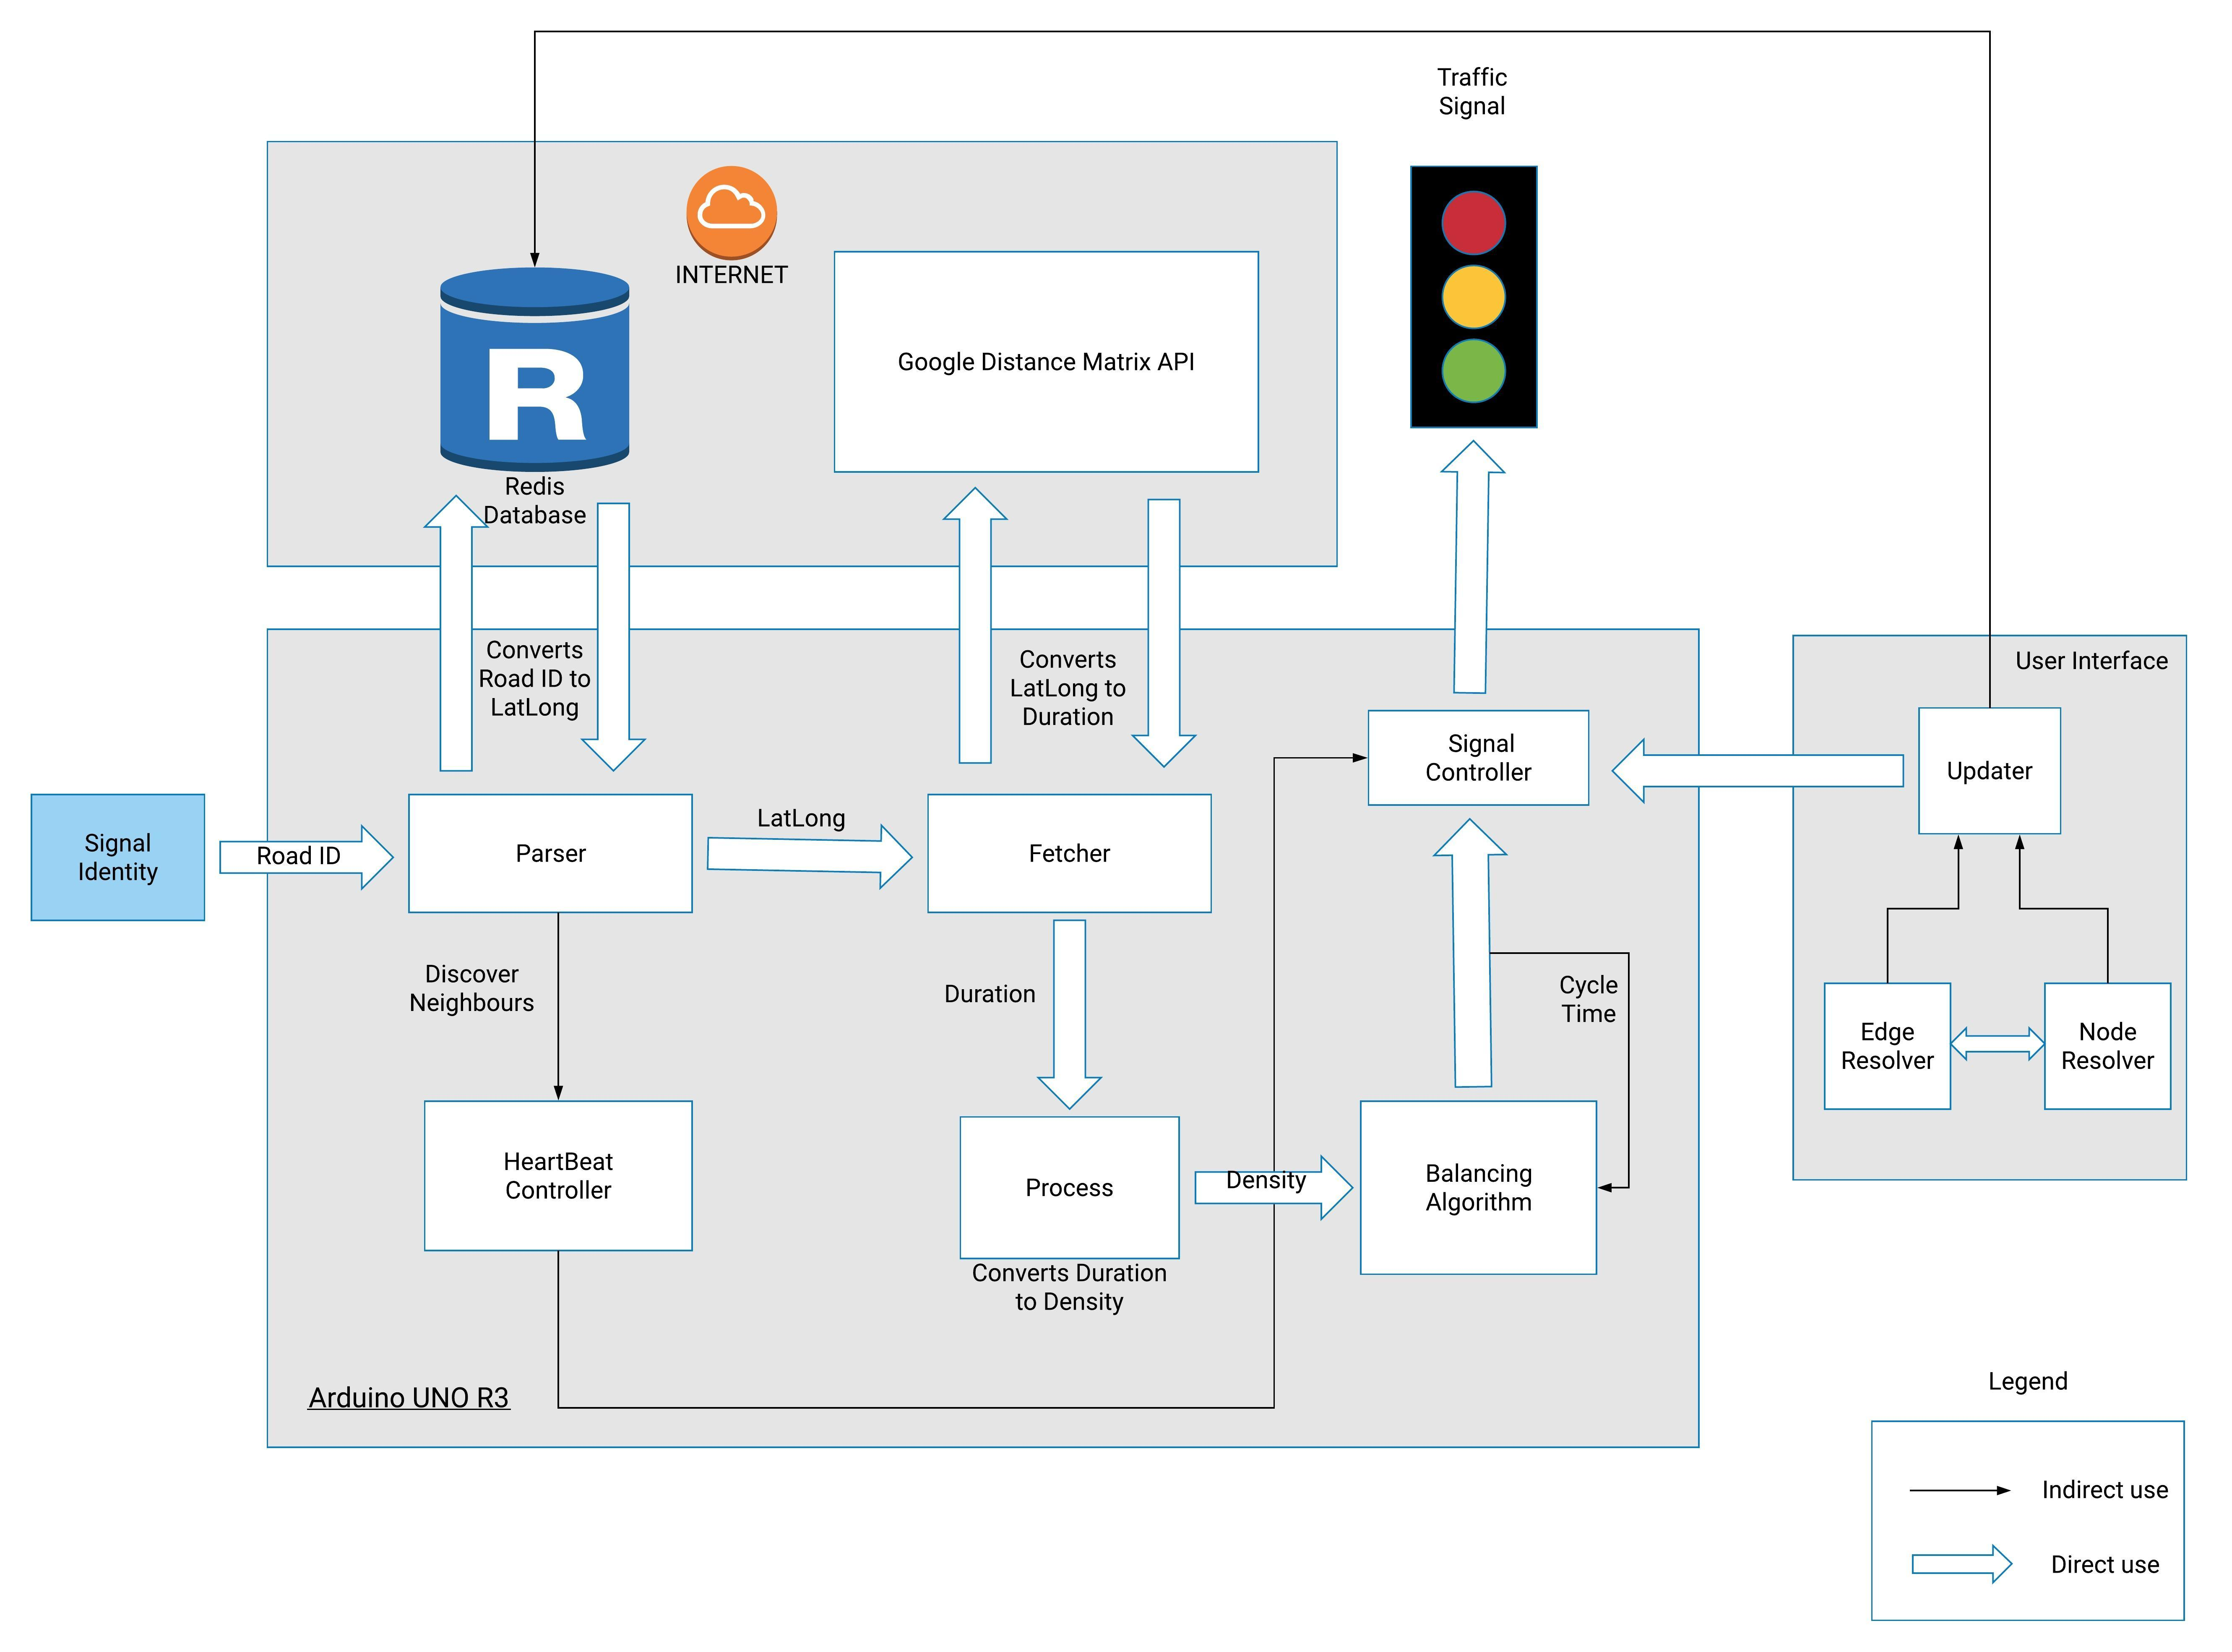
\includegraphics[scale=0.35]{Diagrams/Architecture_Diagram.jpg}
    	\end{center}
    	\caption{Architecture Diagram}
    \end{figure}

\newpage
\section{Software Requirement Specification (SRS)}
\subsection{Interface Requirements:}
\underline{User interfaces:}
\begin{enumerate}
	\item UI for visitors to see signal timings.
	\item UI for authentication of Traffic Control Administrators.
	\item UI for editing (with support for undo/redo) routes and signal operation.
	\item Exposed API for using non-authenticated functionalities outside of UI.
\end{enumerate}

\underline{Hardware Interfaces}
\begin{enumerate}
	\item A hidden P2P communication strategy for real-time monitoring network status.
	\item Automatic route expansion in case of signal controller failure.
\end{enumerate}
\underline{Software Interfaces:}
\begin{enumerate}
	\item Hidden P2P localhost server for notifying lane neighbours.
	\item Web server to Controller interface for operating on controller (switching on/off, changing route, watching timings).
\end{enumerate}

\underline{Communication Interfaces:}
\begin{enumerate}
	\item 3G/4G GSM internet connection.
	\item IoT connectivity between signal controllers.
\end{enumerate}

\newpage


\section{Risk assessment}  
%%what to do?


\newpage
\chapter{Modelling}
\section{UML diagrams} 
\subsection{Structural Diagrams}
\subsubsection{Class Diagram}
	\begin{figure}[!h]
		\begin{center}
			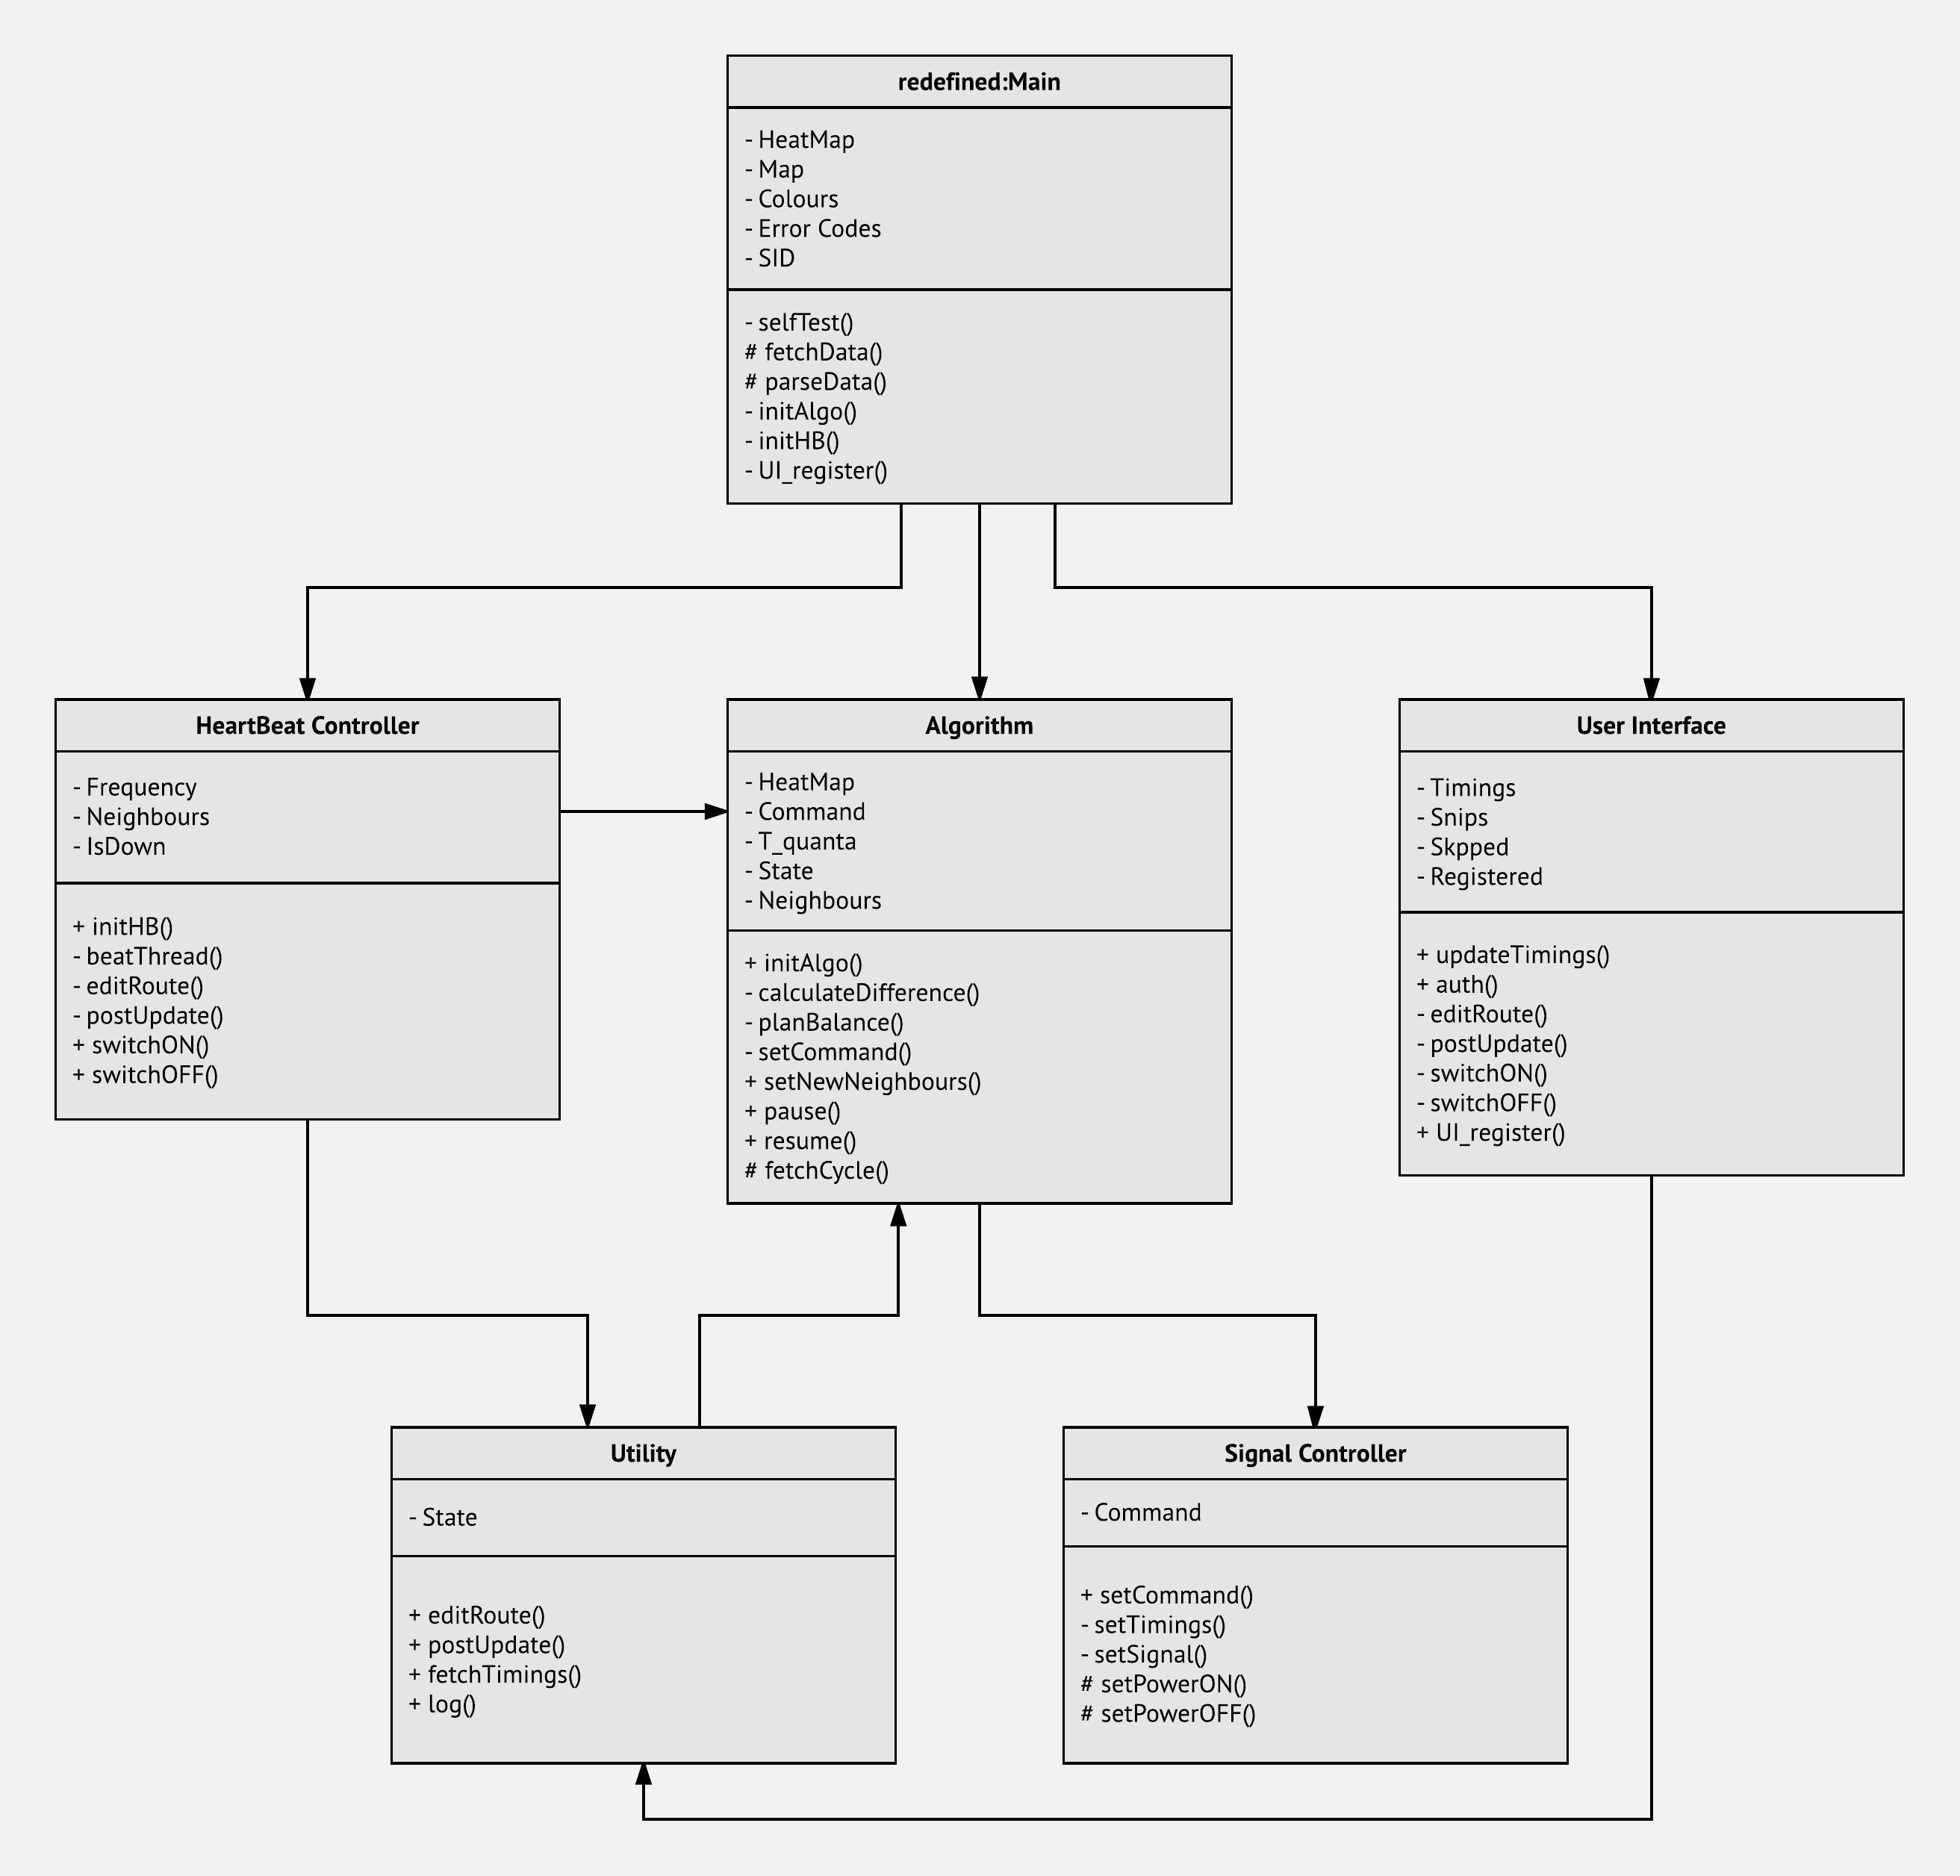
\includegraphics[scale=0.6]{Diagrams/Class_Diagram.jpeg}
		\end{center}
		\caption{Class Diagram.}
	\end{figure}
\newpage
\subsubsection{Object Diagram}
	\begin{figure}[!h]
		\begin{center}
			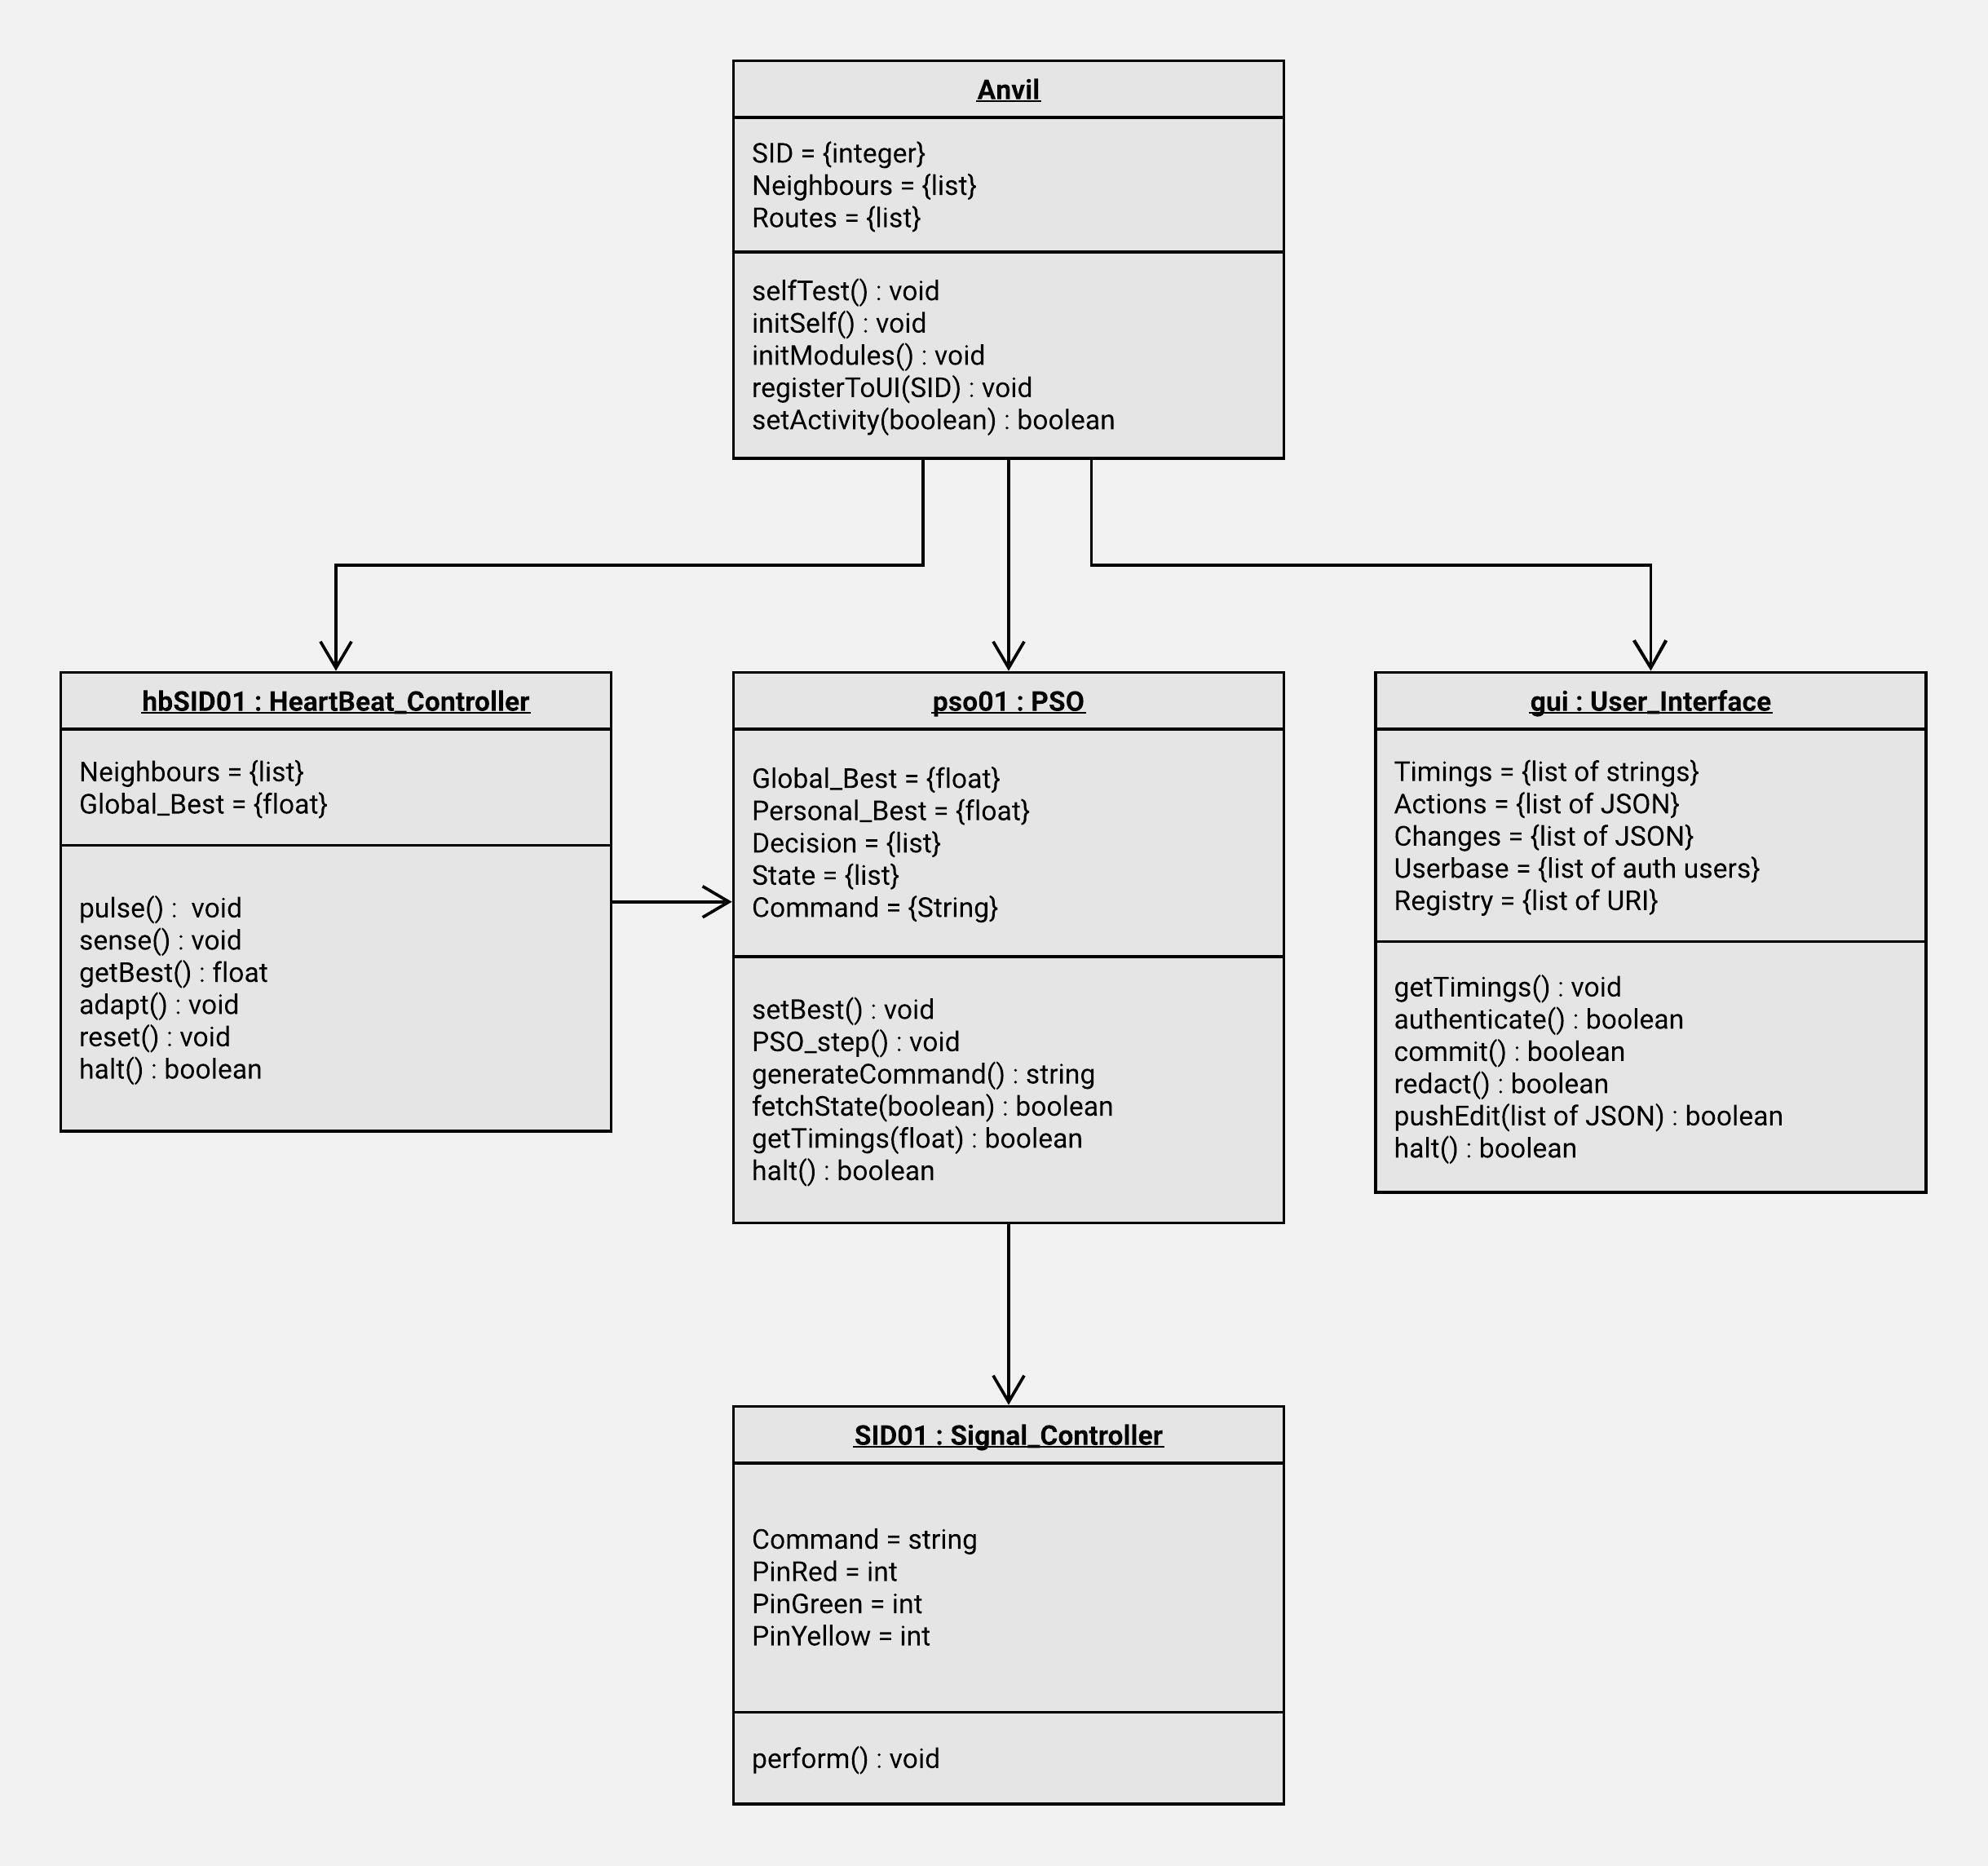
\includegraphics[scale=0.6]{Diagrams/Object_Diagram.jpeg}
		\end{center}
		\caption{Object Diagram.}
	\end{figure}
\newpage
\subsubsection{Component Diagram}
	\begin{figure}[!h]
		\begin{center}
			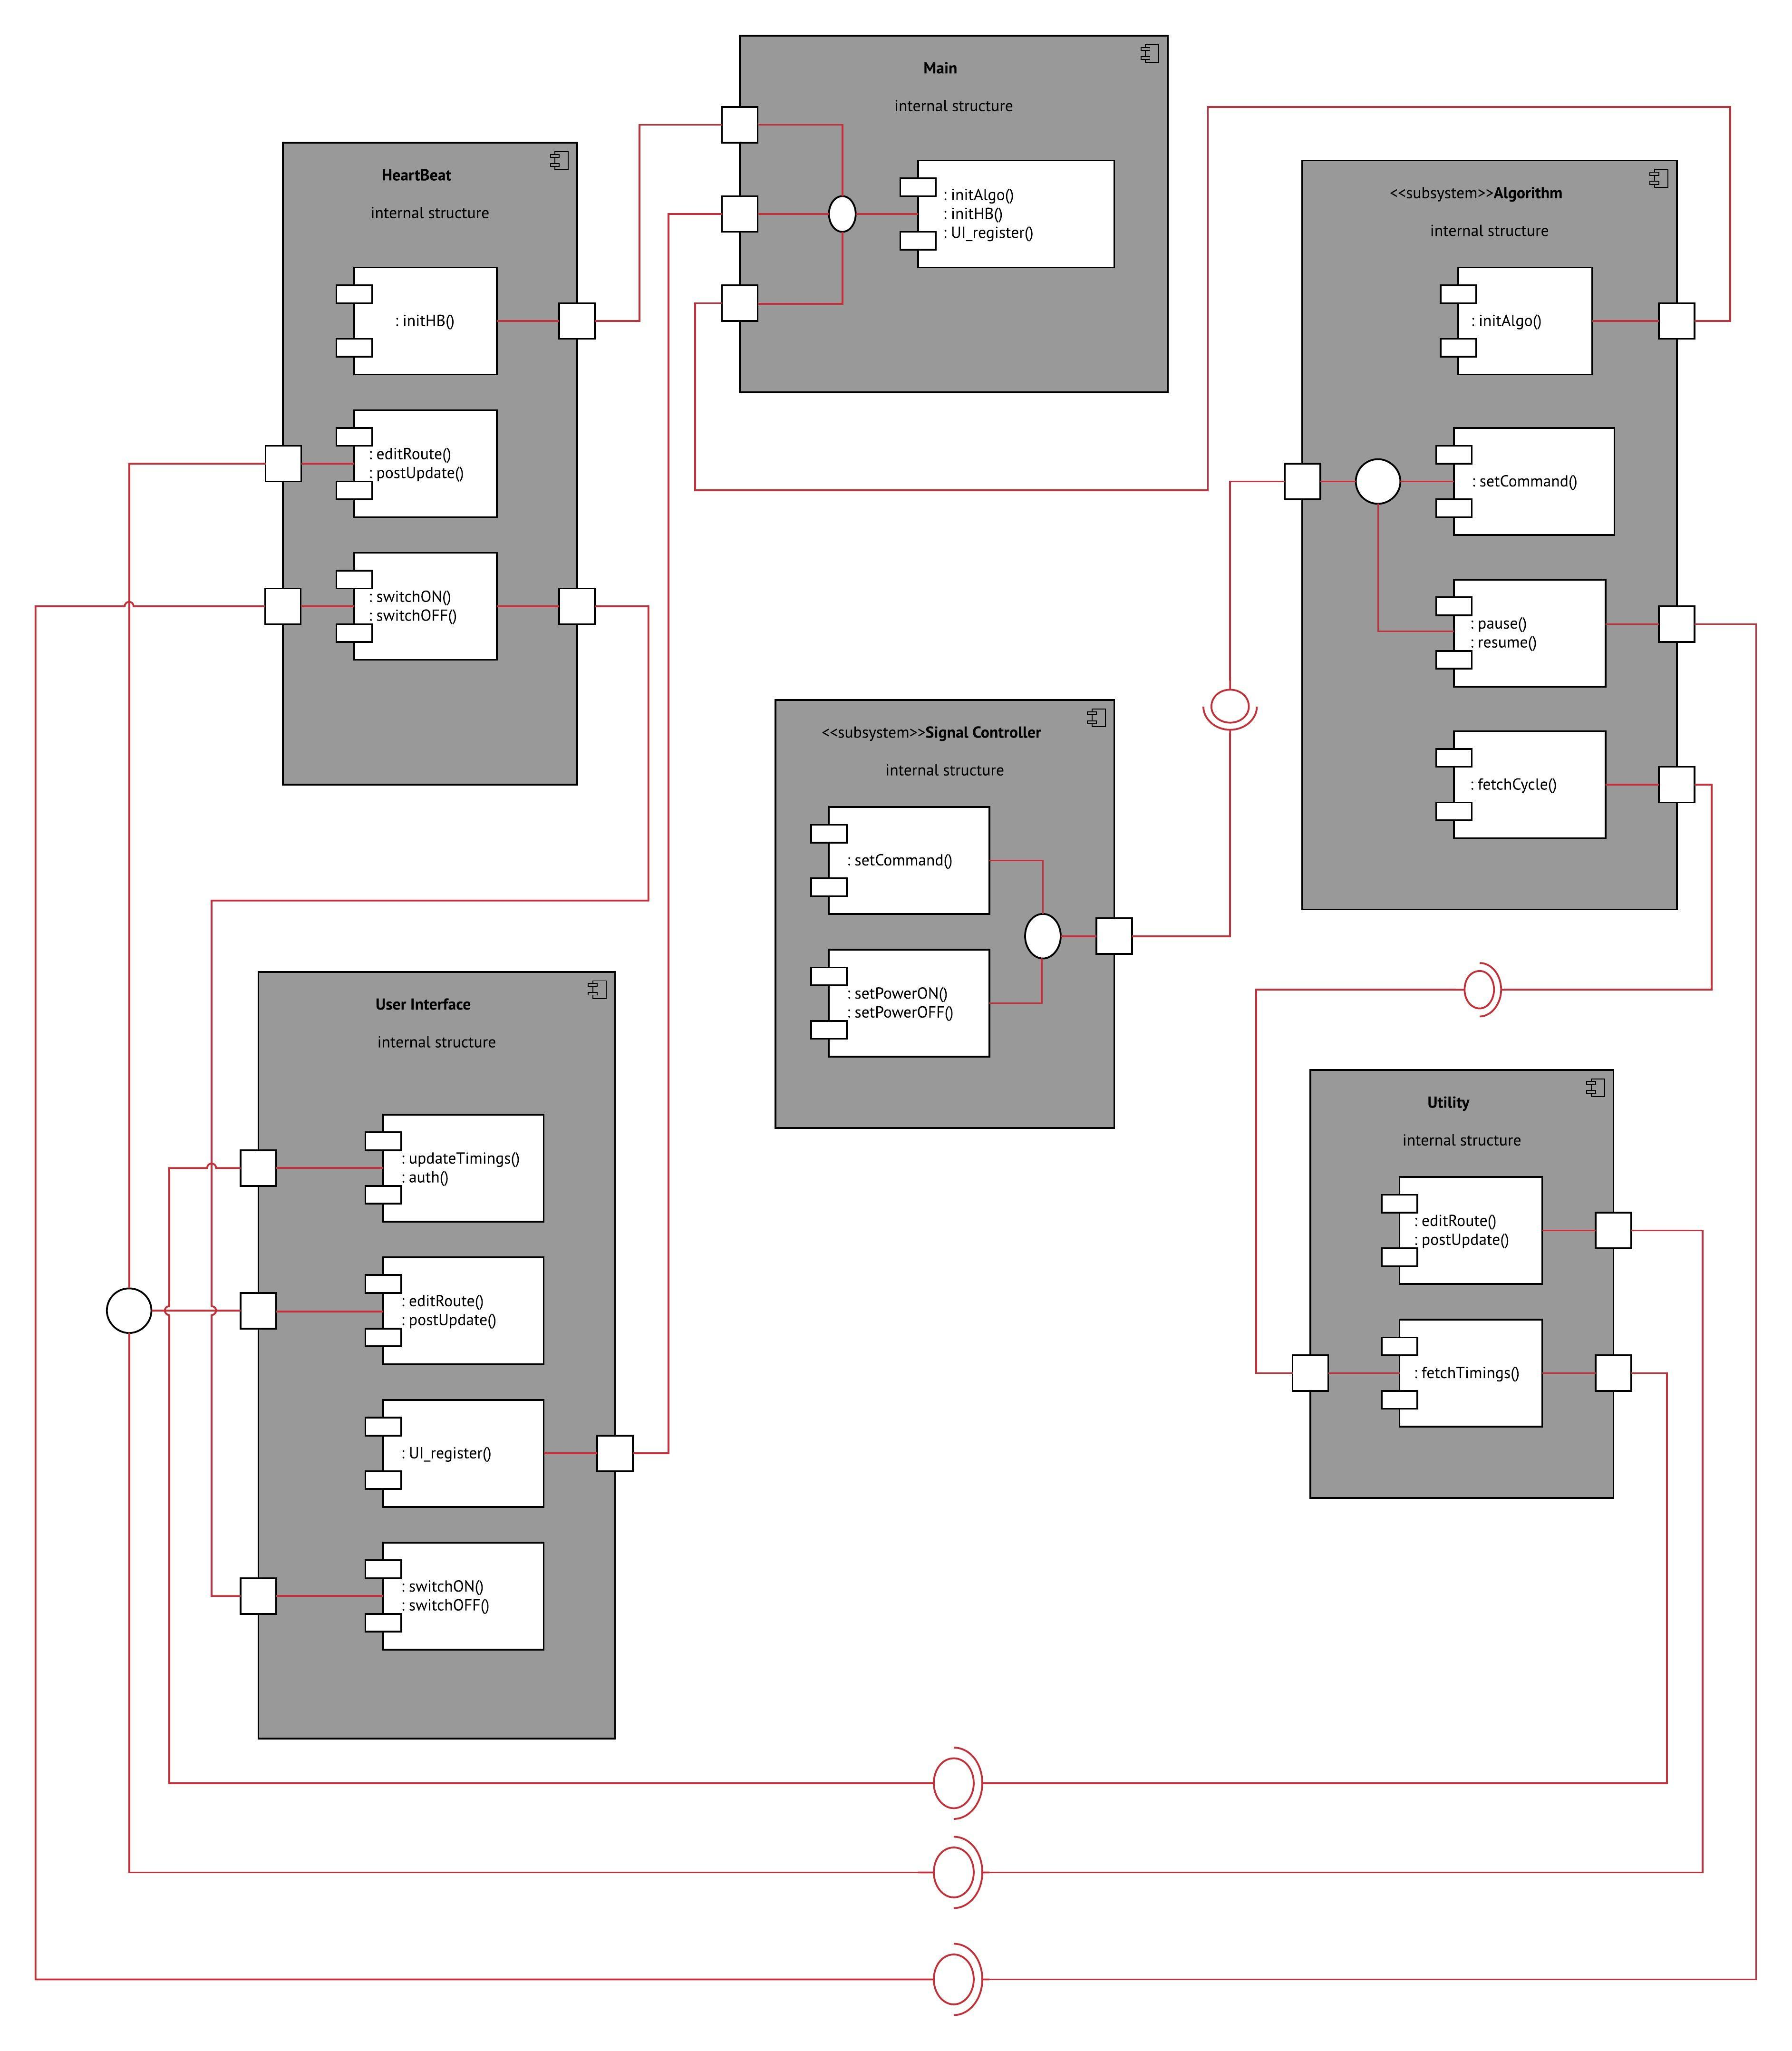
\includegraphics[scale=0.4]{Diagrams/Component_Diagram.jpeg}
		\end{center}
		\caption{Component Diagram.}
	\end{figure}
\newpage
\subsection{Behavioural Diagrams}

\subsubsection{Use Case Diagram}
	\begin{figure}[!h]
		\begin{center}
			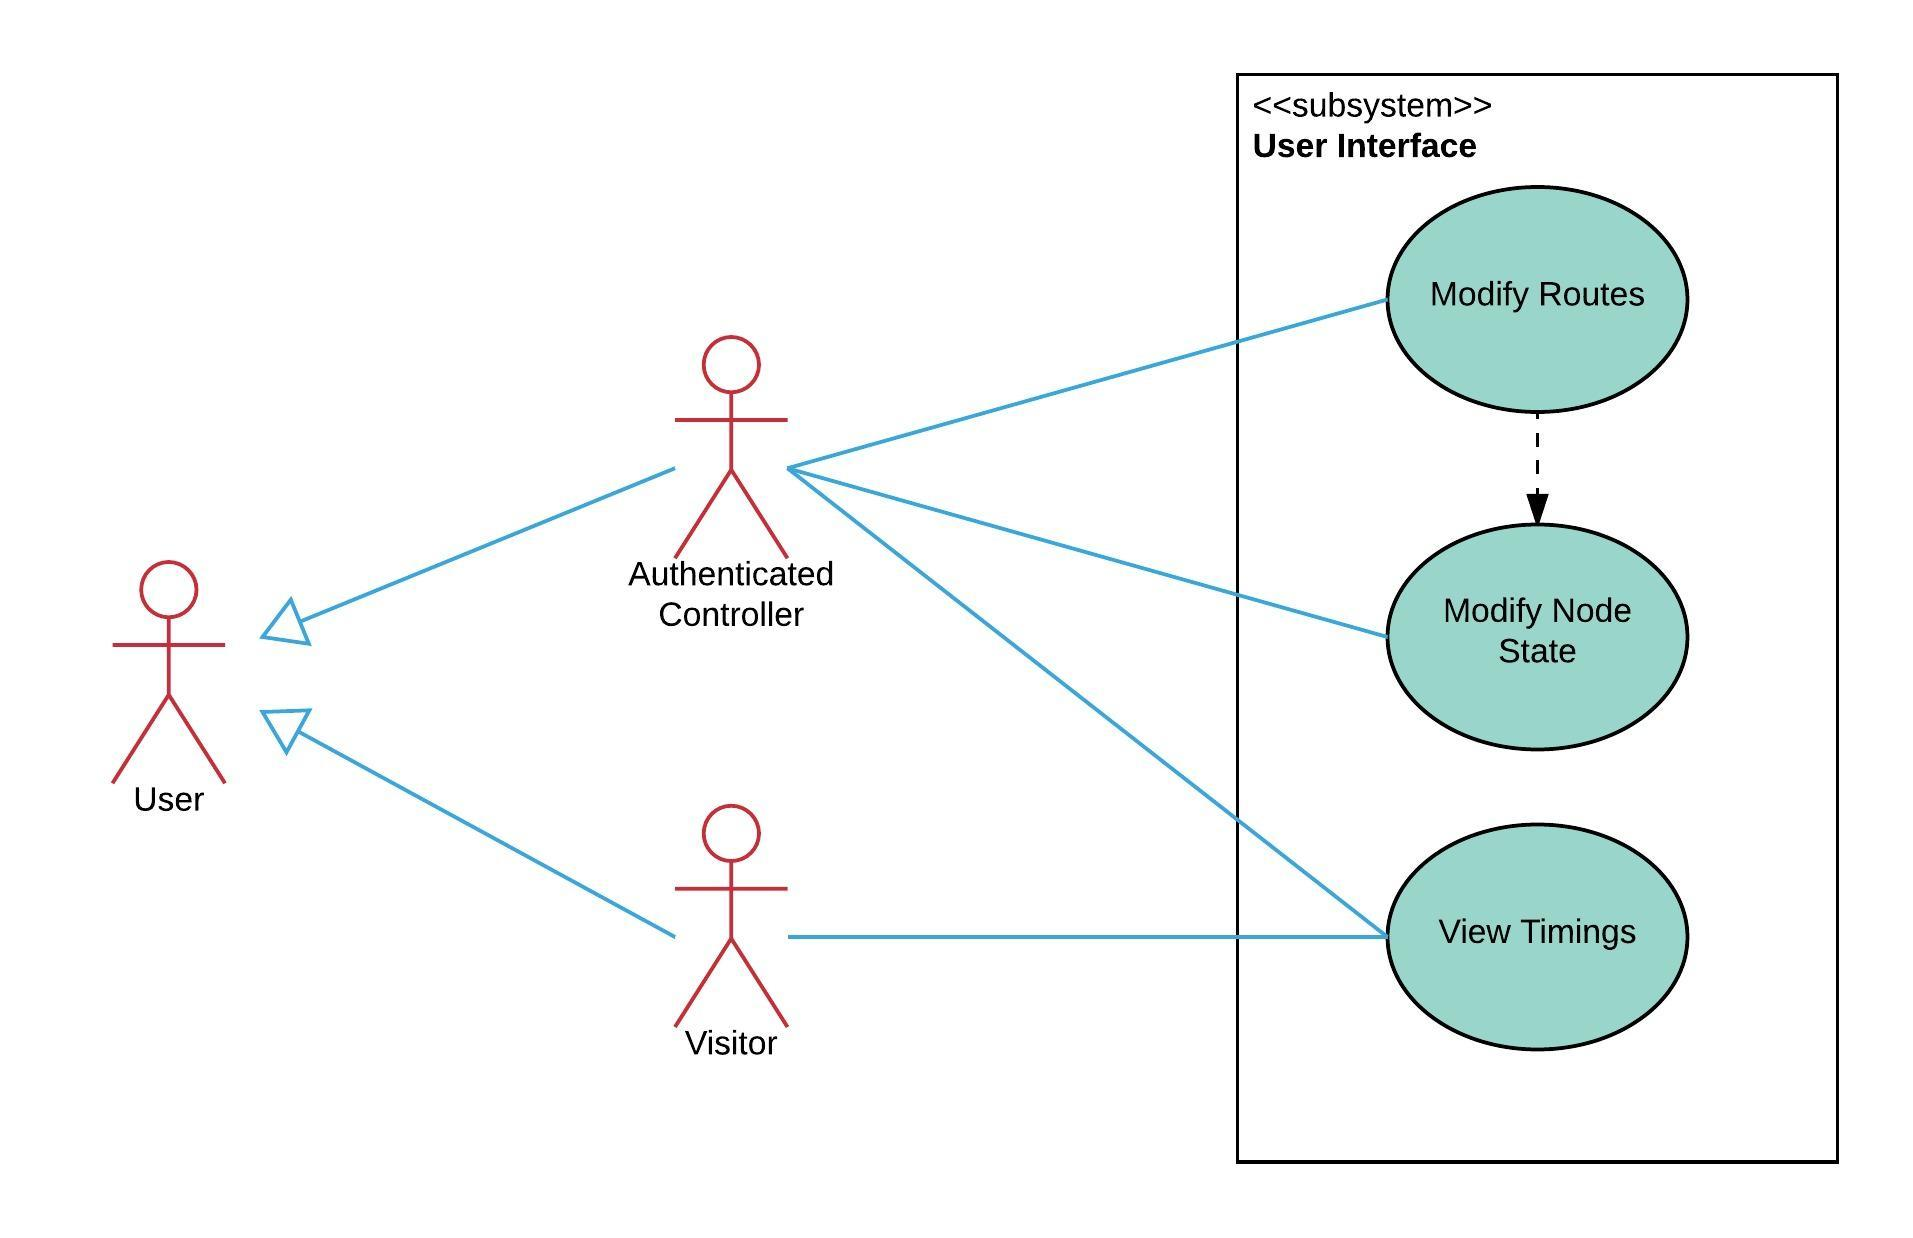
\includegraphics[scale=0.2]{Diagrams/Use_Case_Diagram.jpeg}
		\end{center}
		\caption{Use Case Diagram.}
	\end{figure}
\newpage
\subsubsection{StateChart Diagram}
	\begin{figure}[!h]
		\begin{center}
			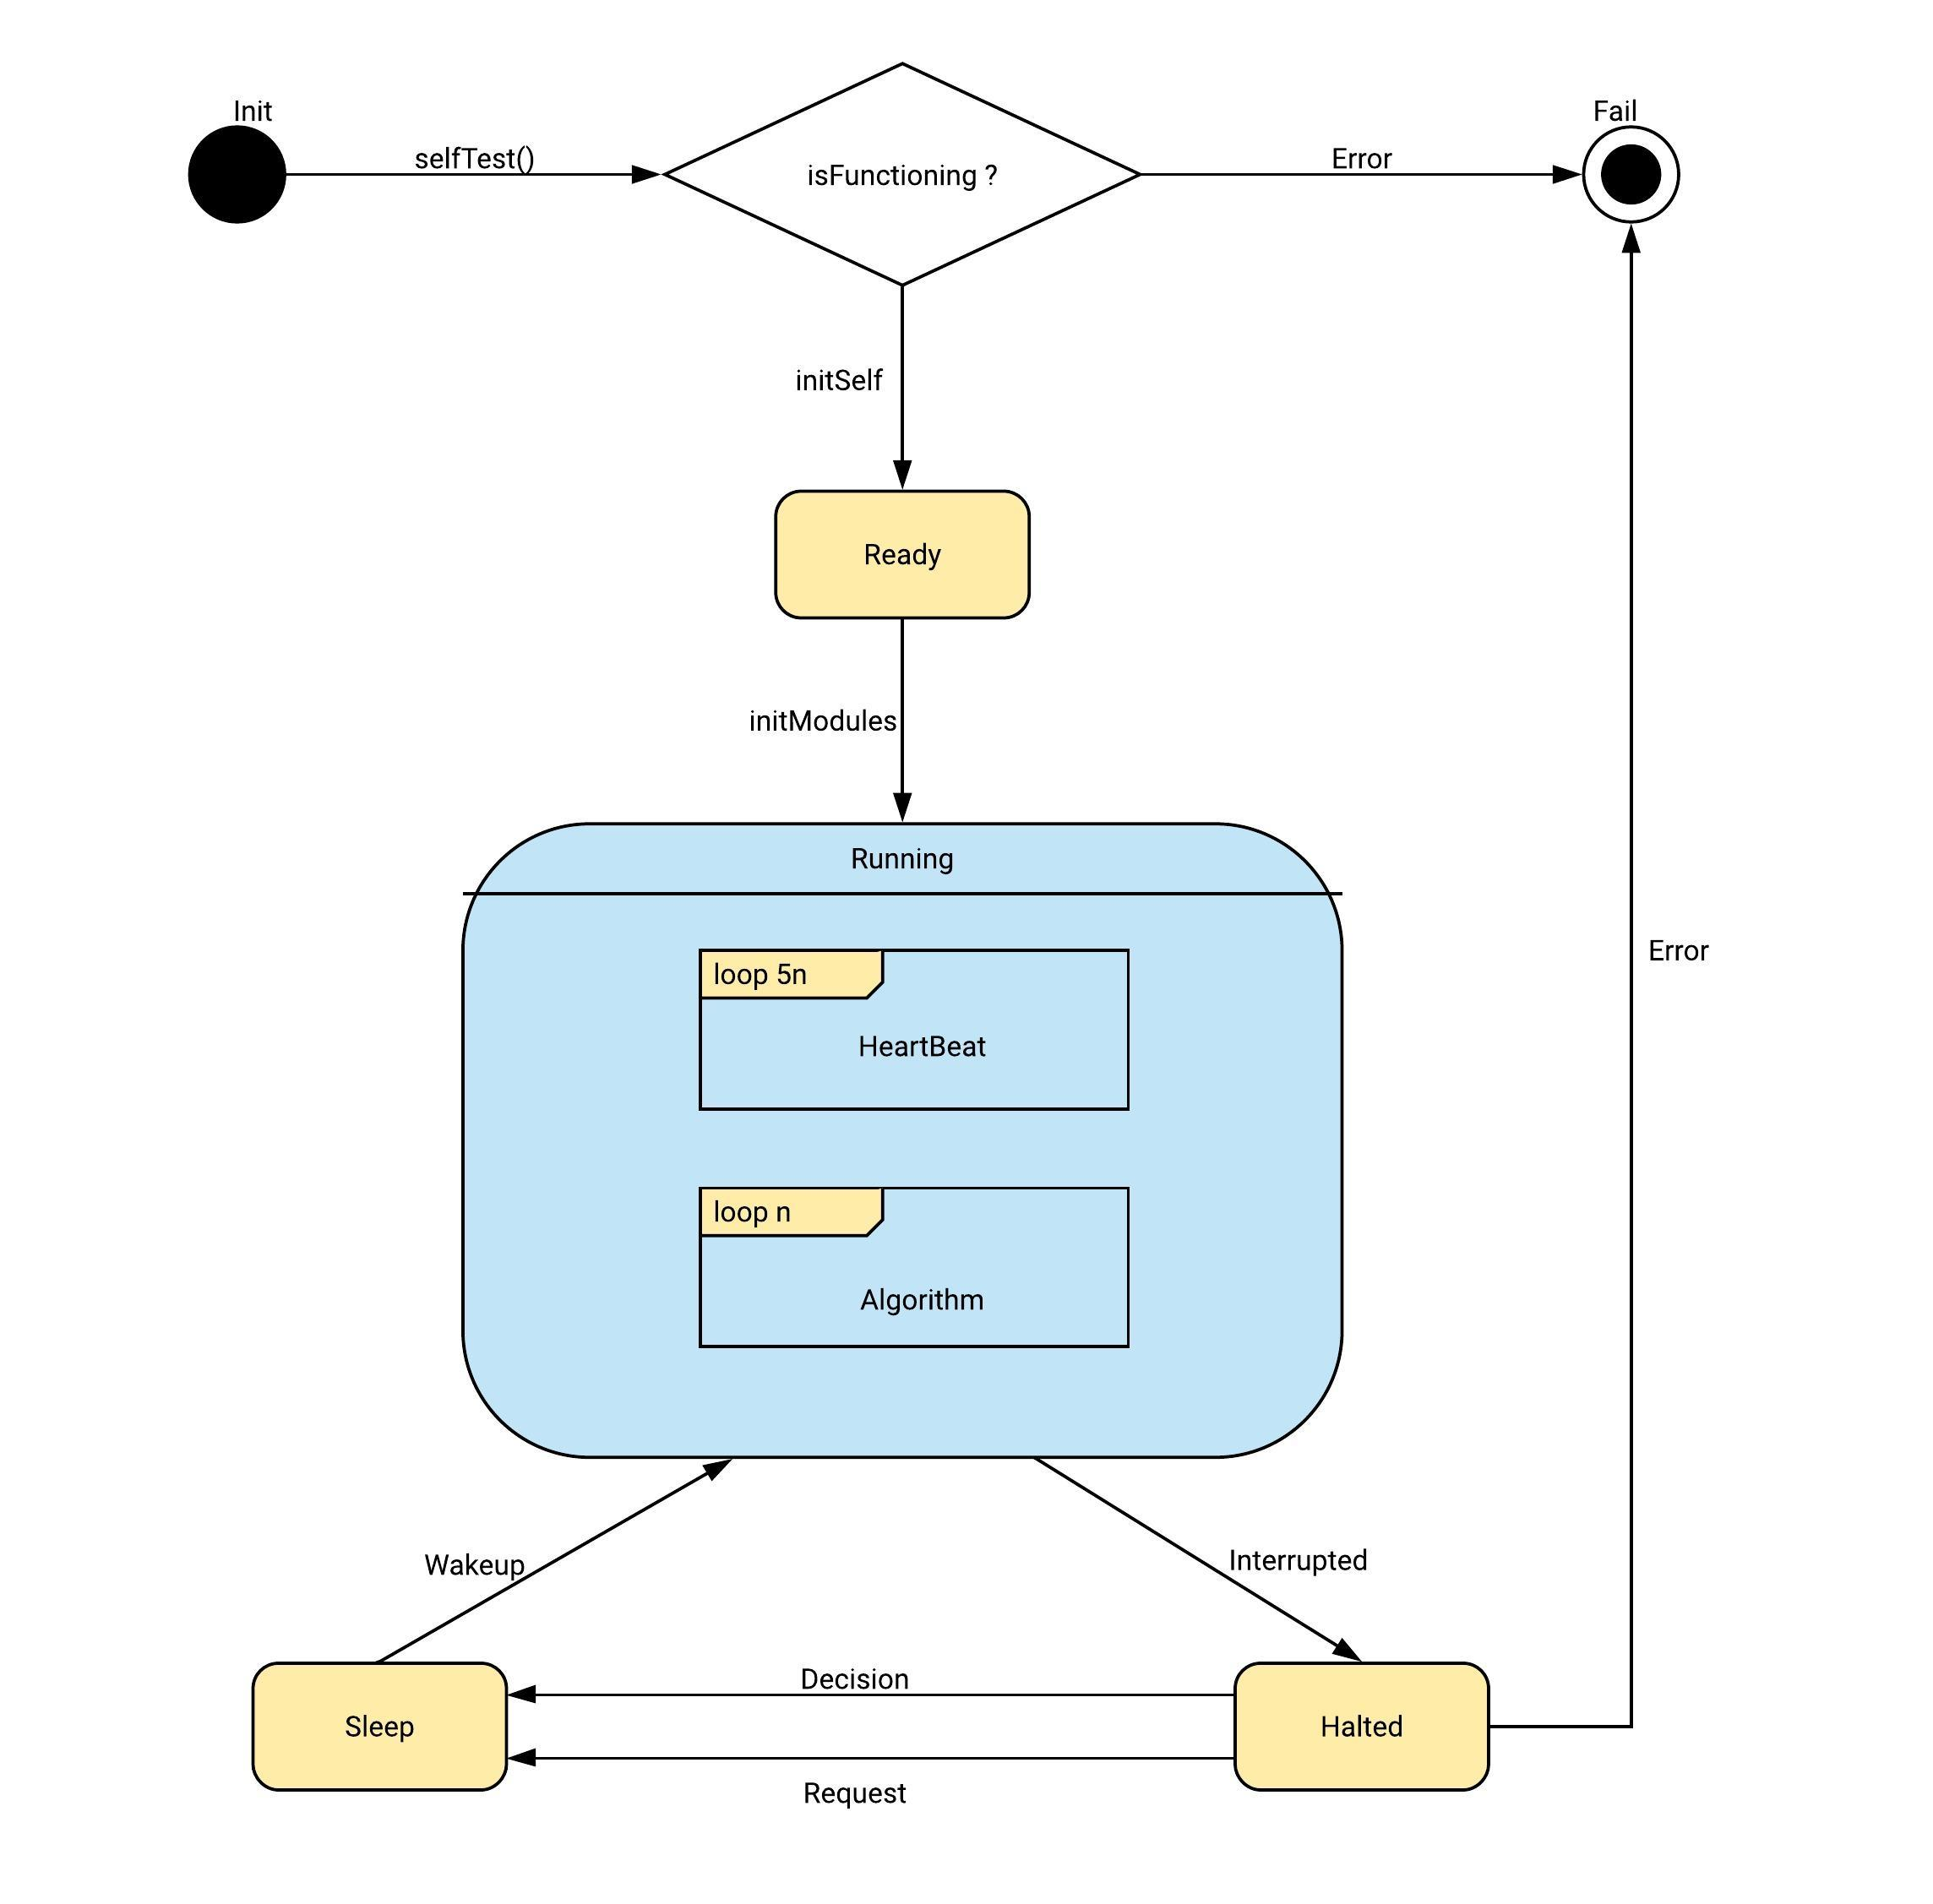
\includegraphics[scale=0.35]{Diagrams/StateChart_Diagram.jpeg}
		\end{center}
		\caption{StateChart Diagram.}
	\end{figure}


\subsubsection{Sequence Diagrams}
	\begin{figure}[!h]
		\begin{center}
			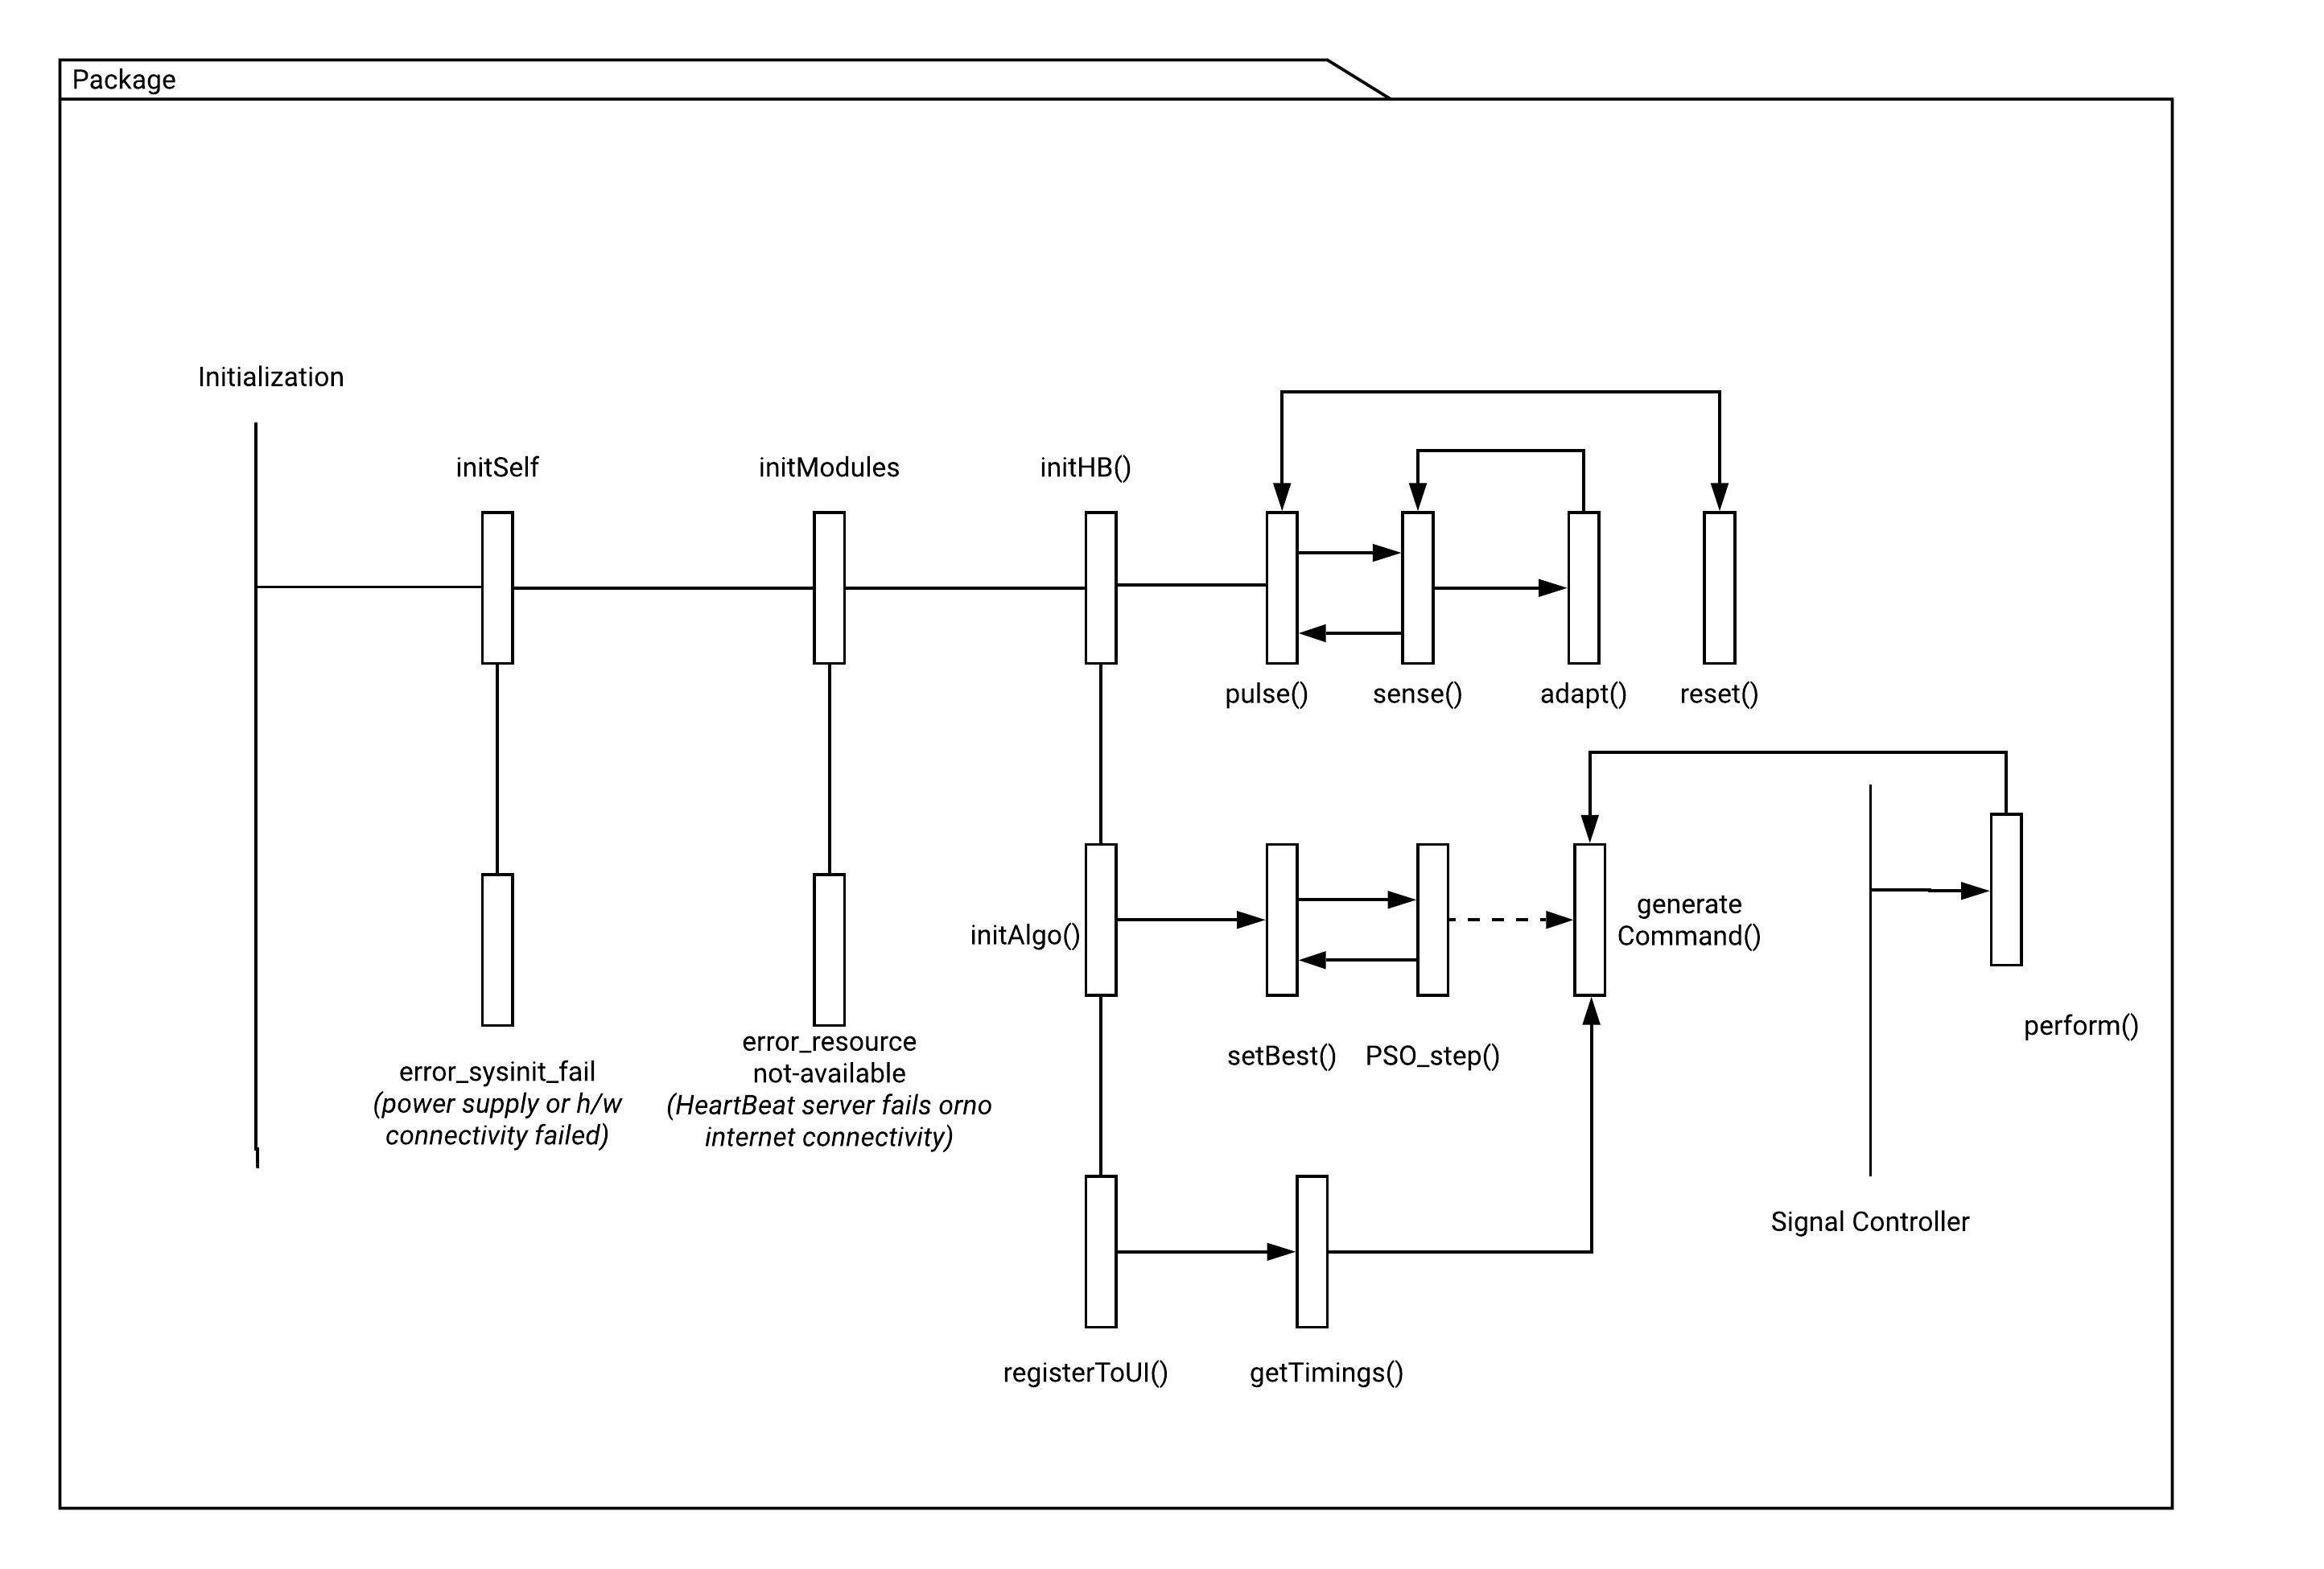
\includegraphics[scale=0.4]{Diagrams/Initialization_Sequence.jpeg}
		\end{center}
		\caption{Initialization Sequence, with support for failure of nearby nodes.}
	\end{figure}
	
\newpage

	\begin{figure}[!h]
		\begin{center}
			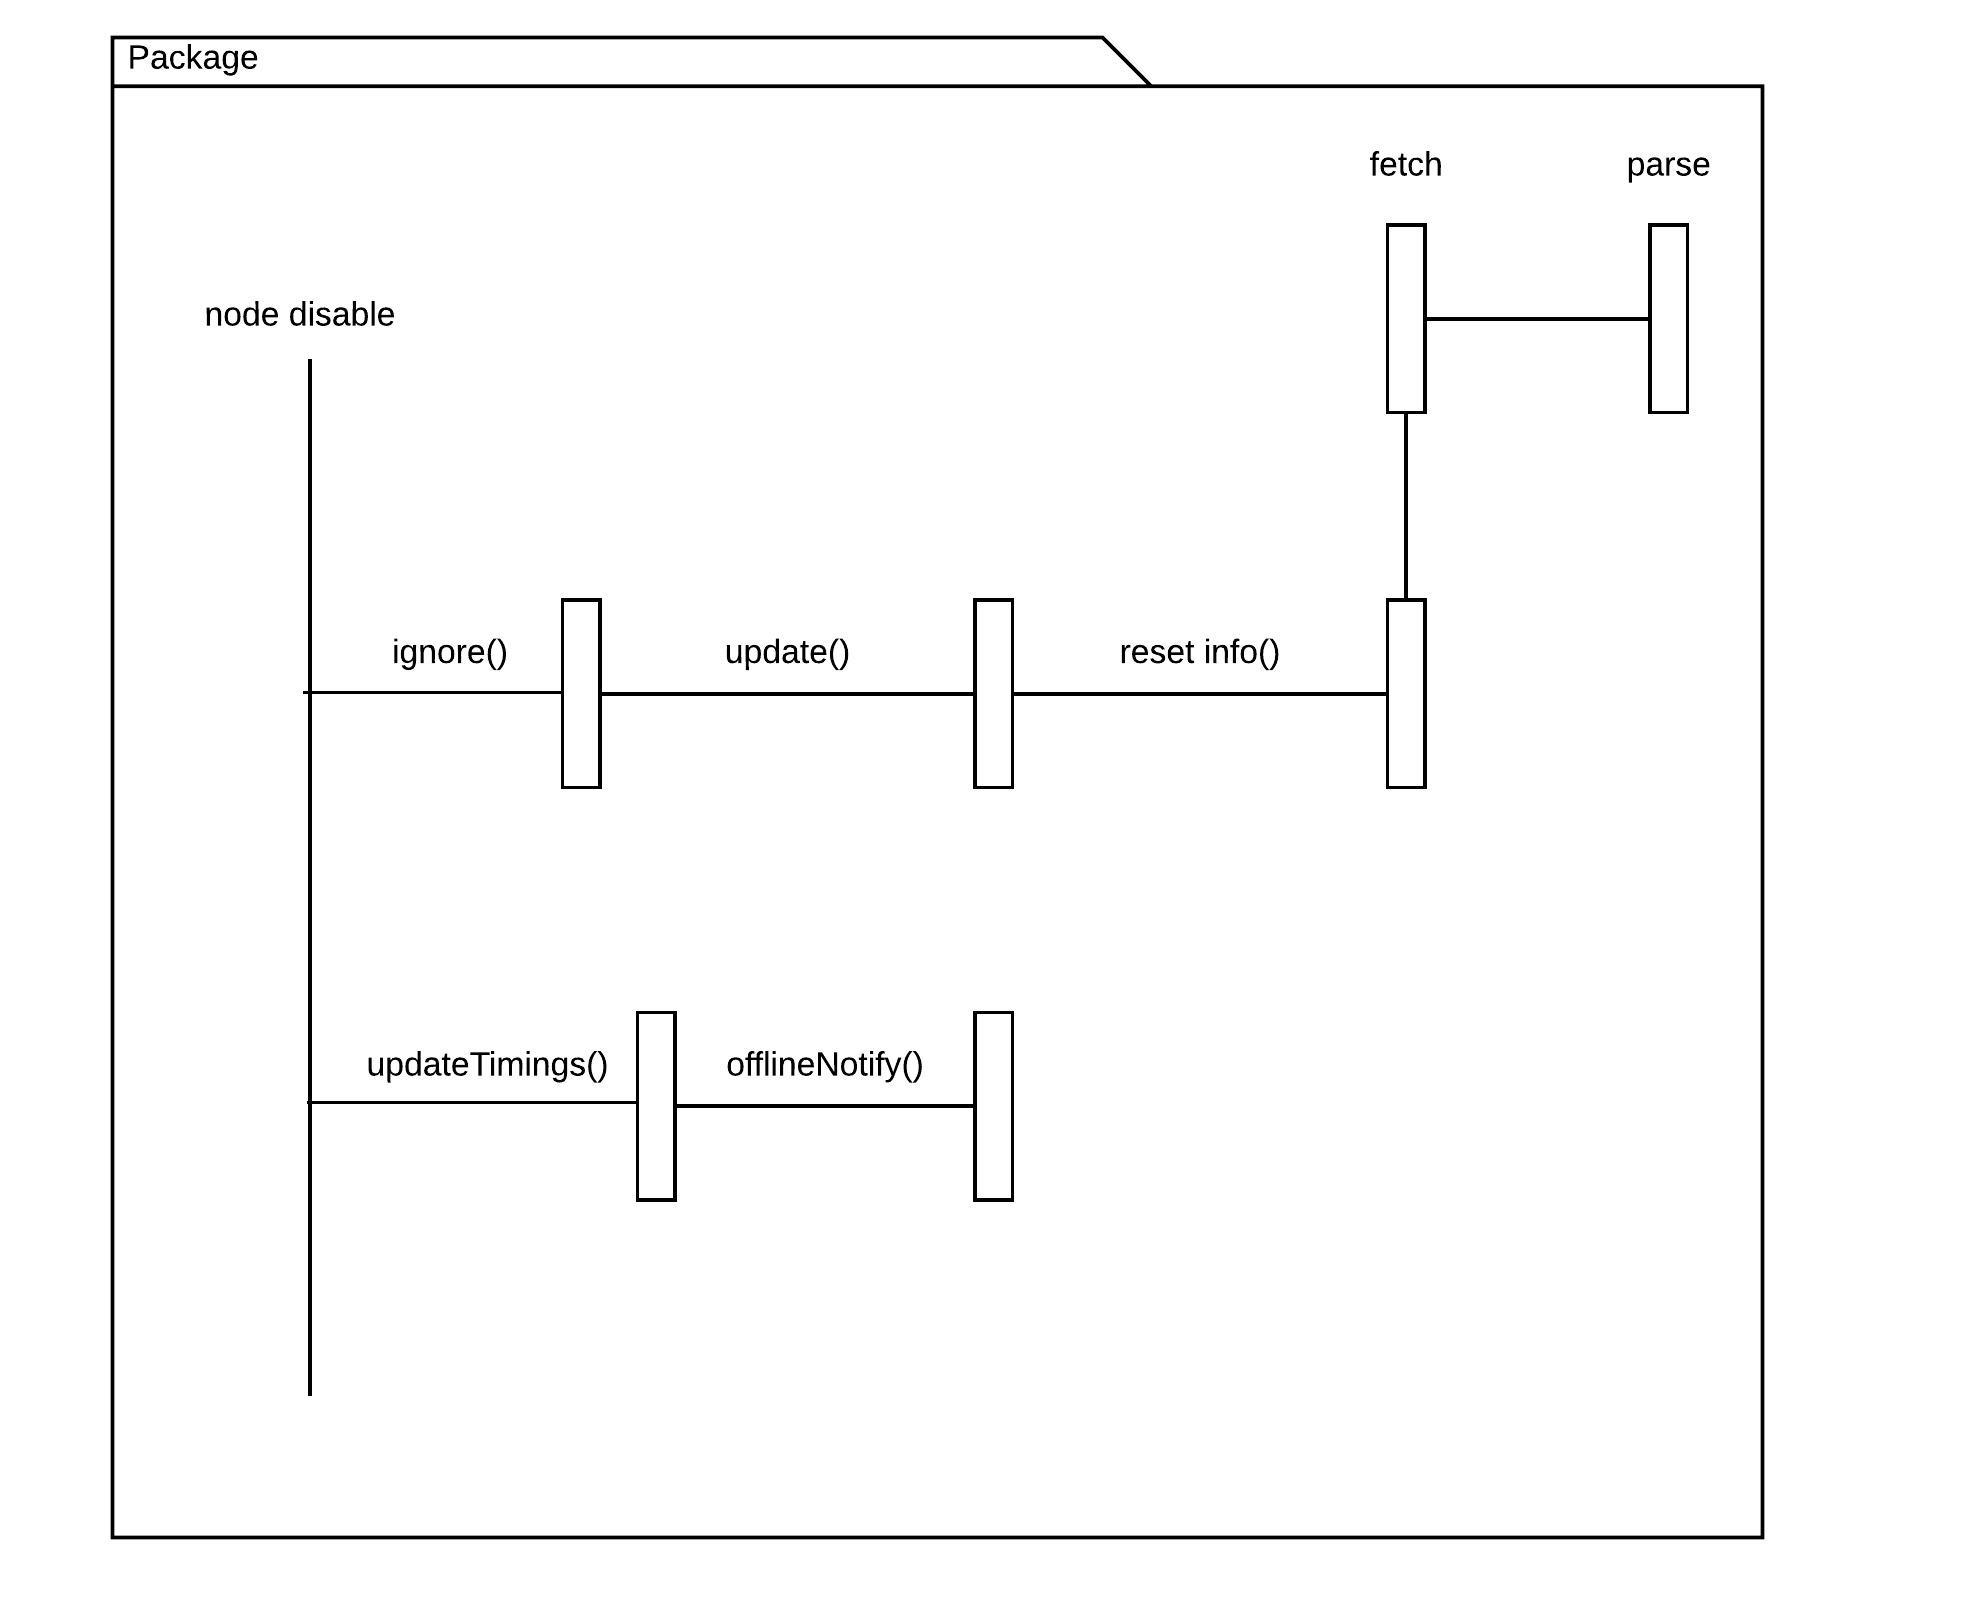
\includegraphics[scale=0.6]{Diagrams/Node_Disable_Sequence.jpeg}
		\end{center}
		\caption{Node Removal Sequence.}
	\end{figure}

	\begin{figure}[!h]
		\begin{center}
			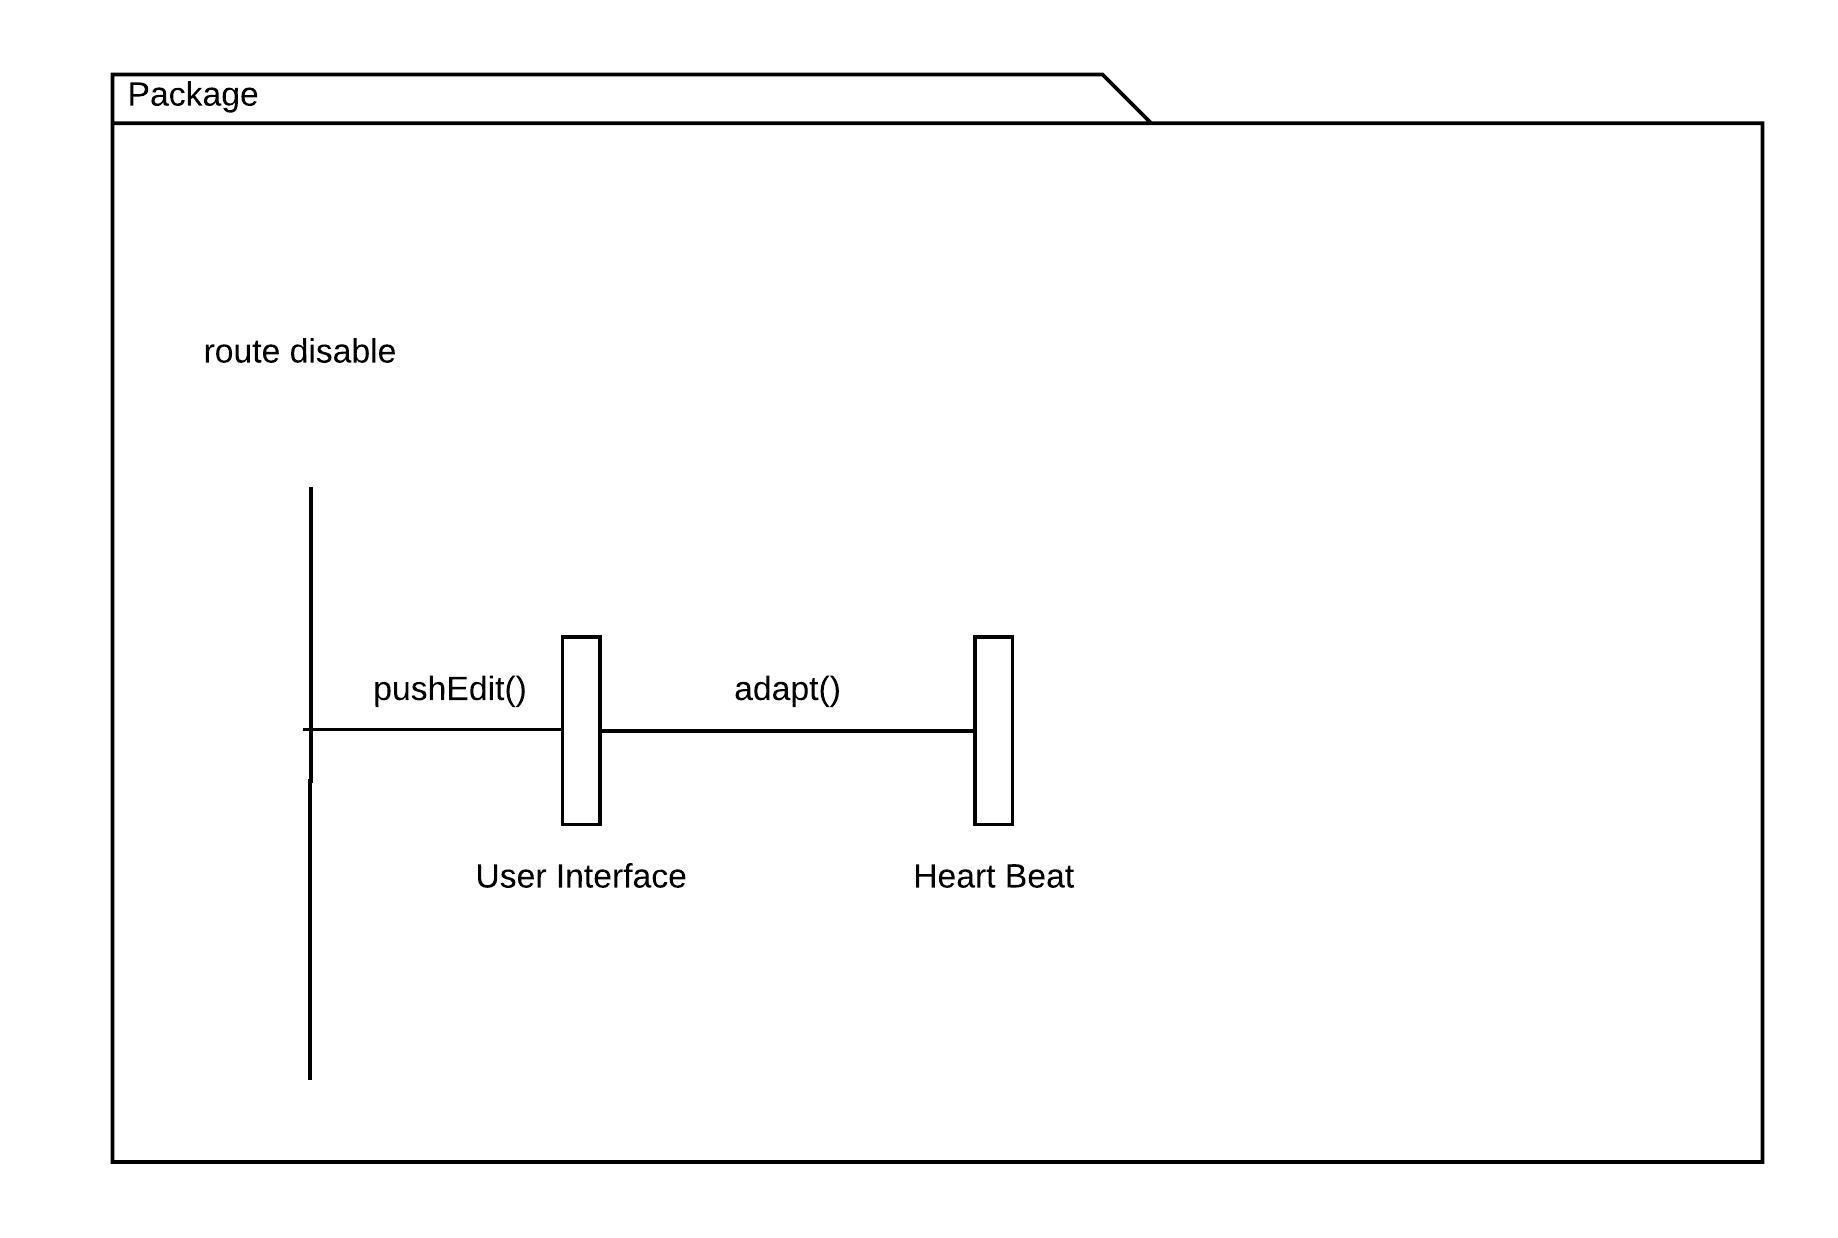
\includegraphics[scale=0.5]{Diagrams/Route_Disable_Sequence.jpeg}
		\end{center}
		\caption{Route Modification Sequence.}
	\end{figure}
		
\newpage

	\begin{figure}[!h]
		\begin{center}
			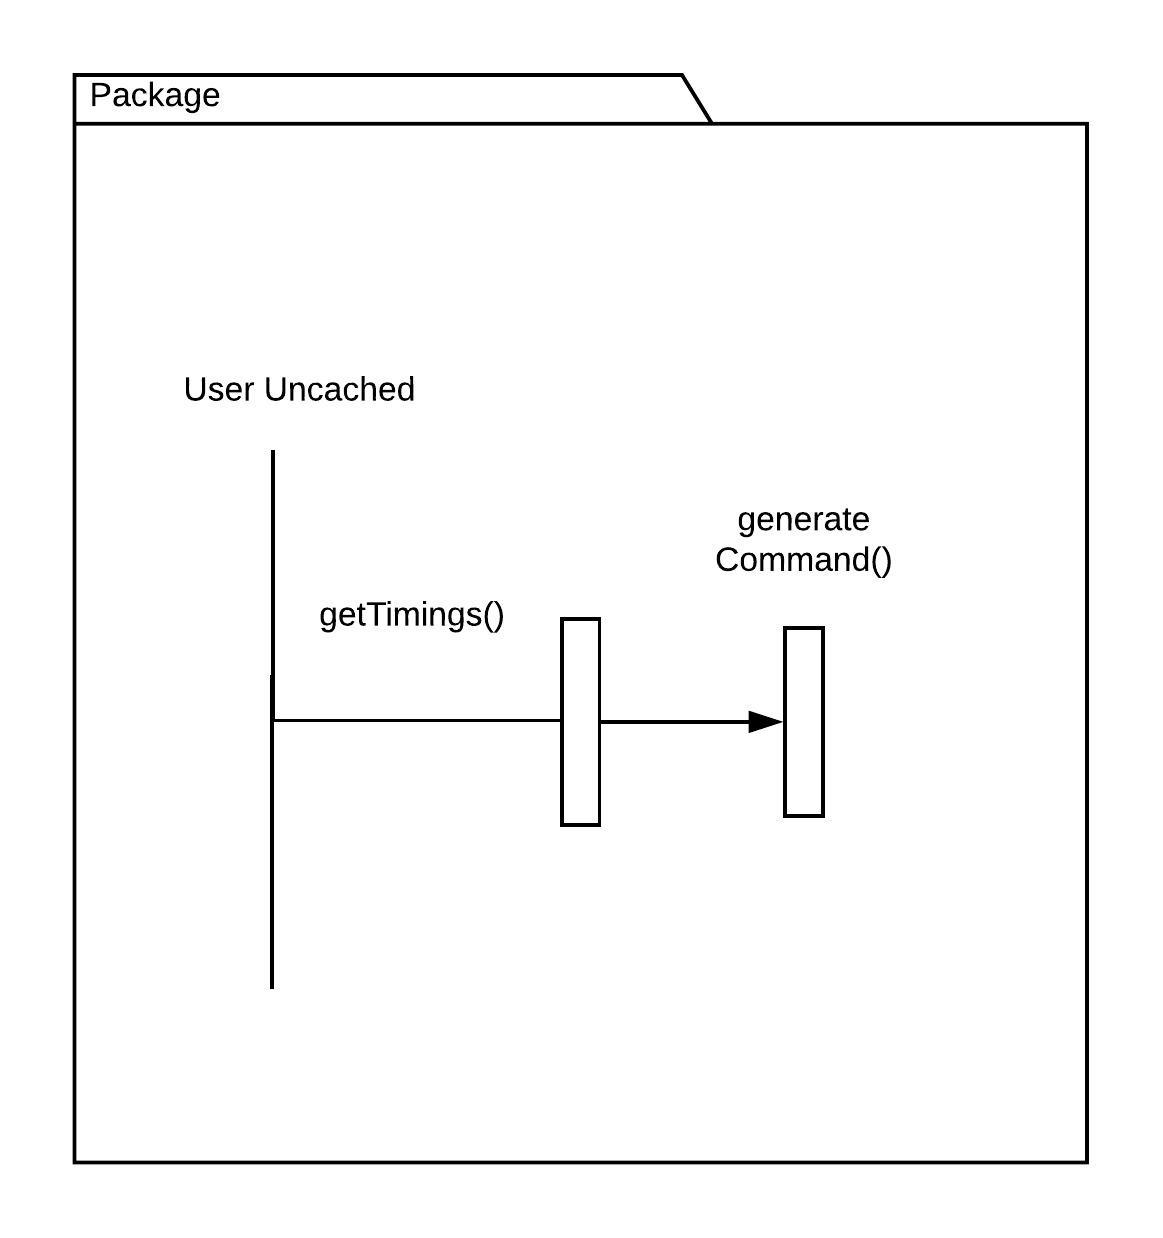
\includegraphics[scale=0.7]{Diagrams/User_View_(Uncached)_Sequence.jpeg}
		\end{center}
		\caption{Visitor's Usage Sequence (uncached data).}
	\end{figure}
	\begin{figure}[!h]
		\begin{center}
			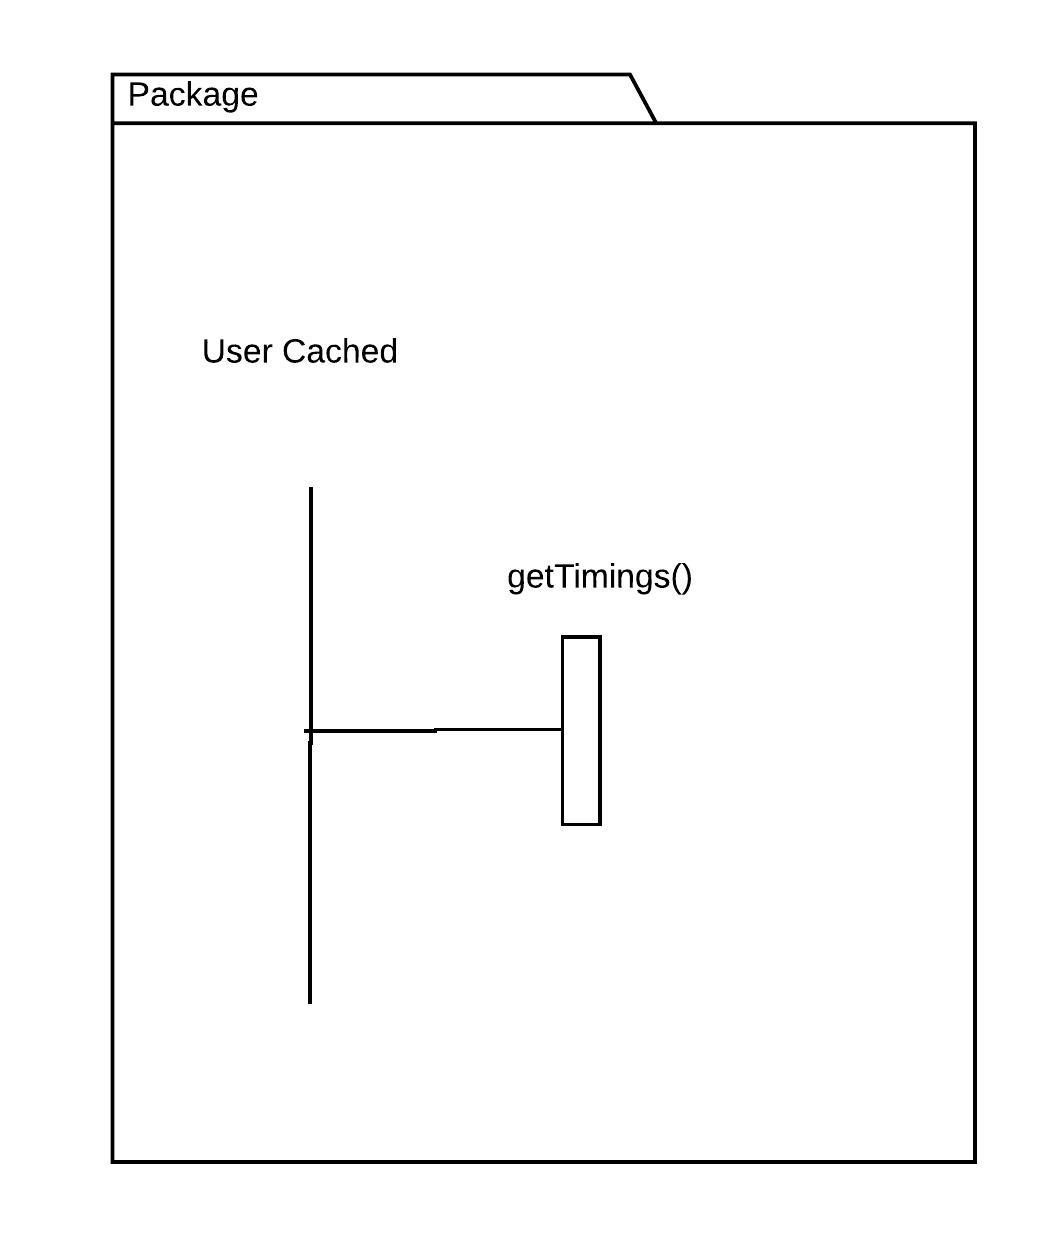
\includegraphics[scale=0.7]{Diagrams/User_View_(Cached)_Sequence.jpeg}
		\end{center}
		\caption{Visitor's Usage Sequence (cached data).}
	\end{figure}
\newpage

\subsubsection{Activity Diagram}
	\begin{figure}[!h]
		\begin{center}
			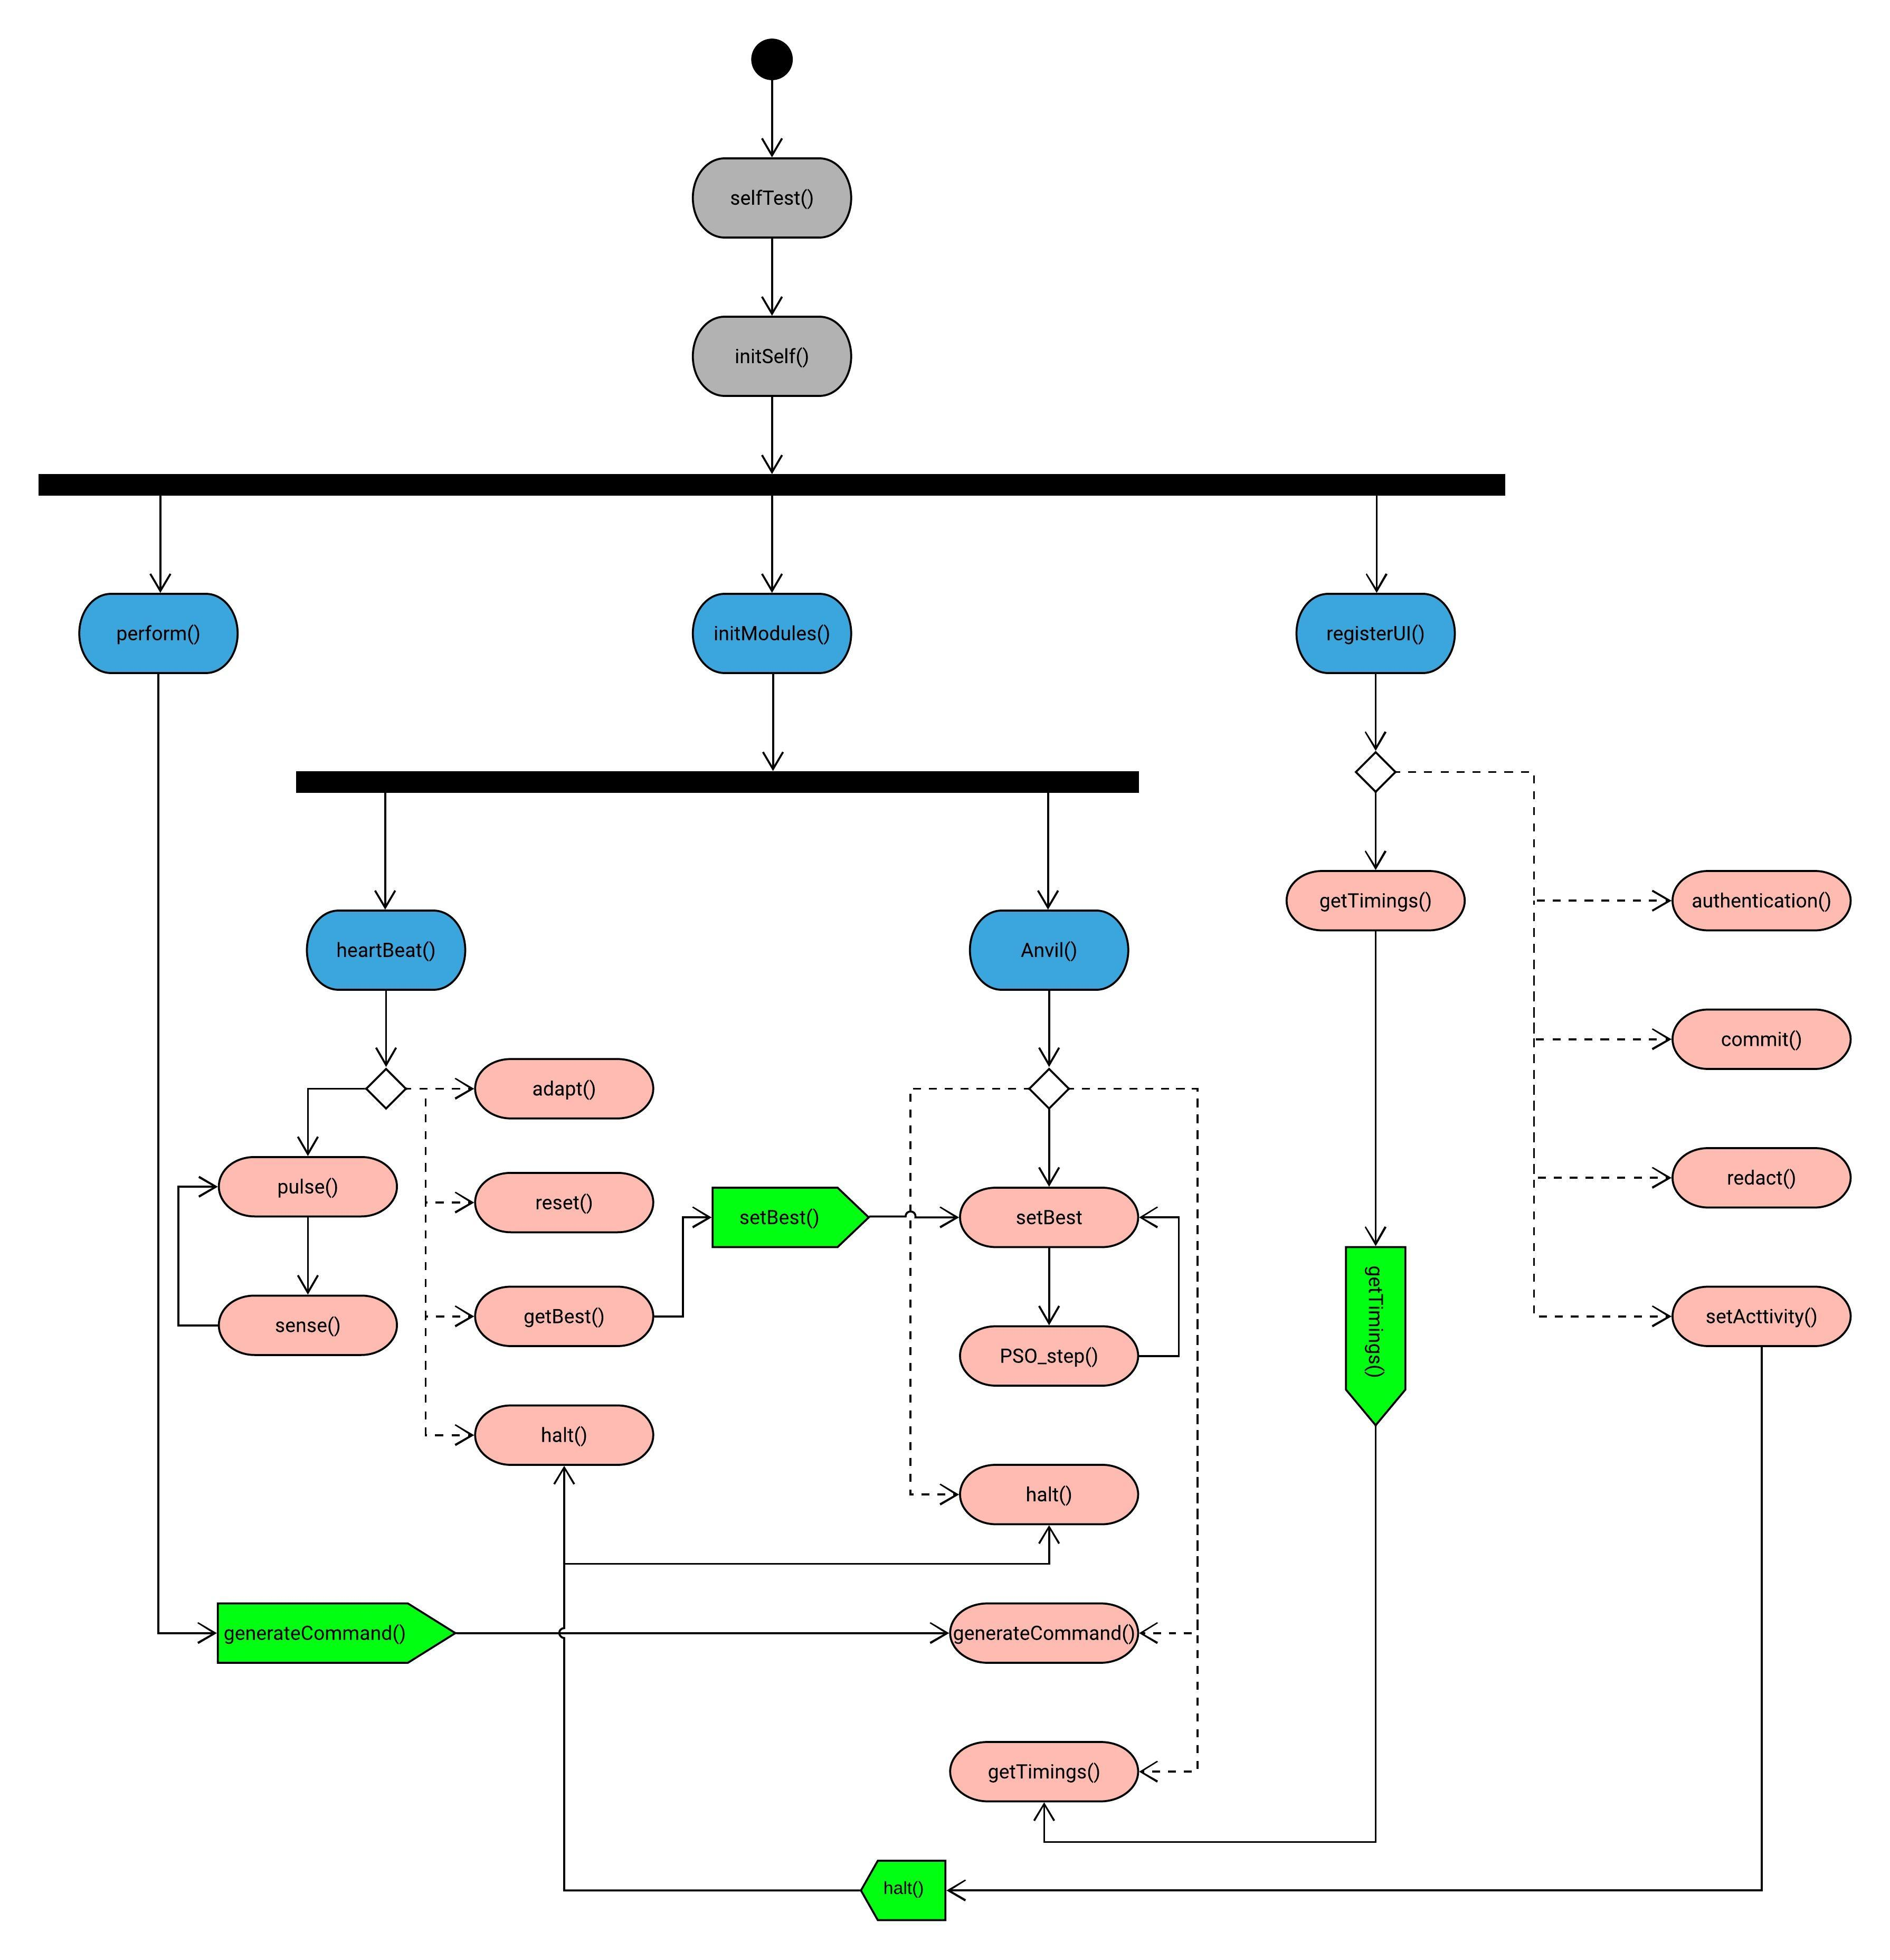
\includegraphics[scale=0.45]{Diagrams/Activity_Diagram.jpeg}
		\end{center}
		\caption{Activity Diagram.}
	\end{figure}


\newpage
\section{ERD and Normalization for database if any}
\subsection{Entity Relationship Diagram}
	\begin{figure}[!ht]
		\begin{center}
			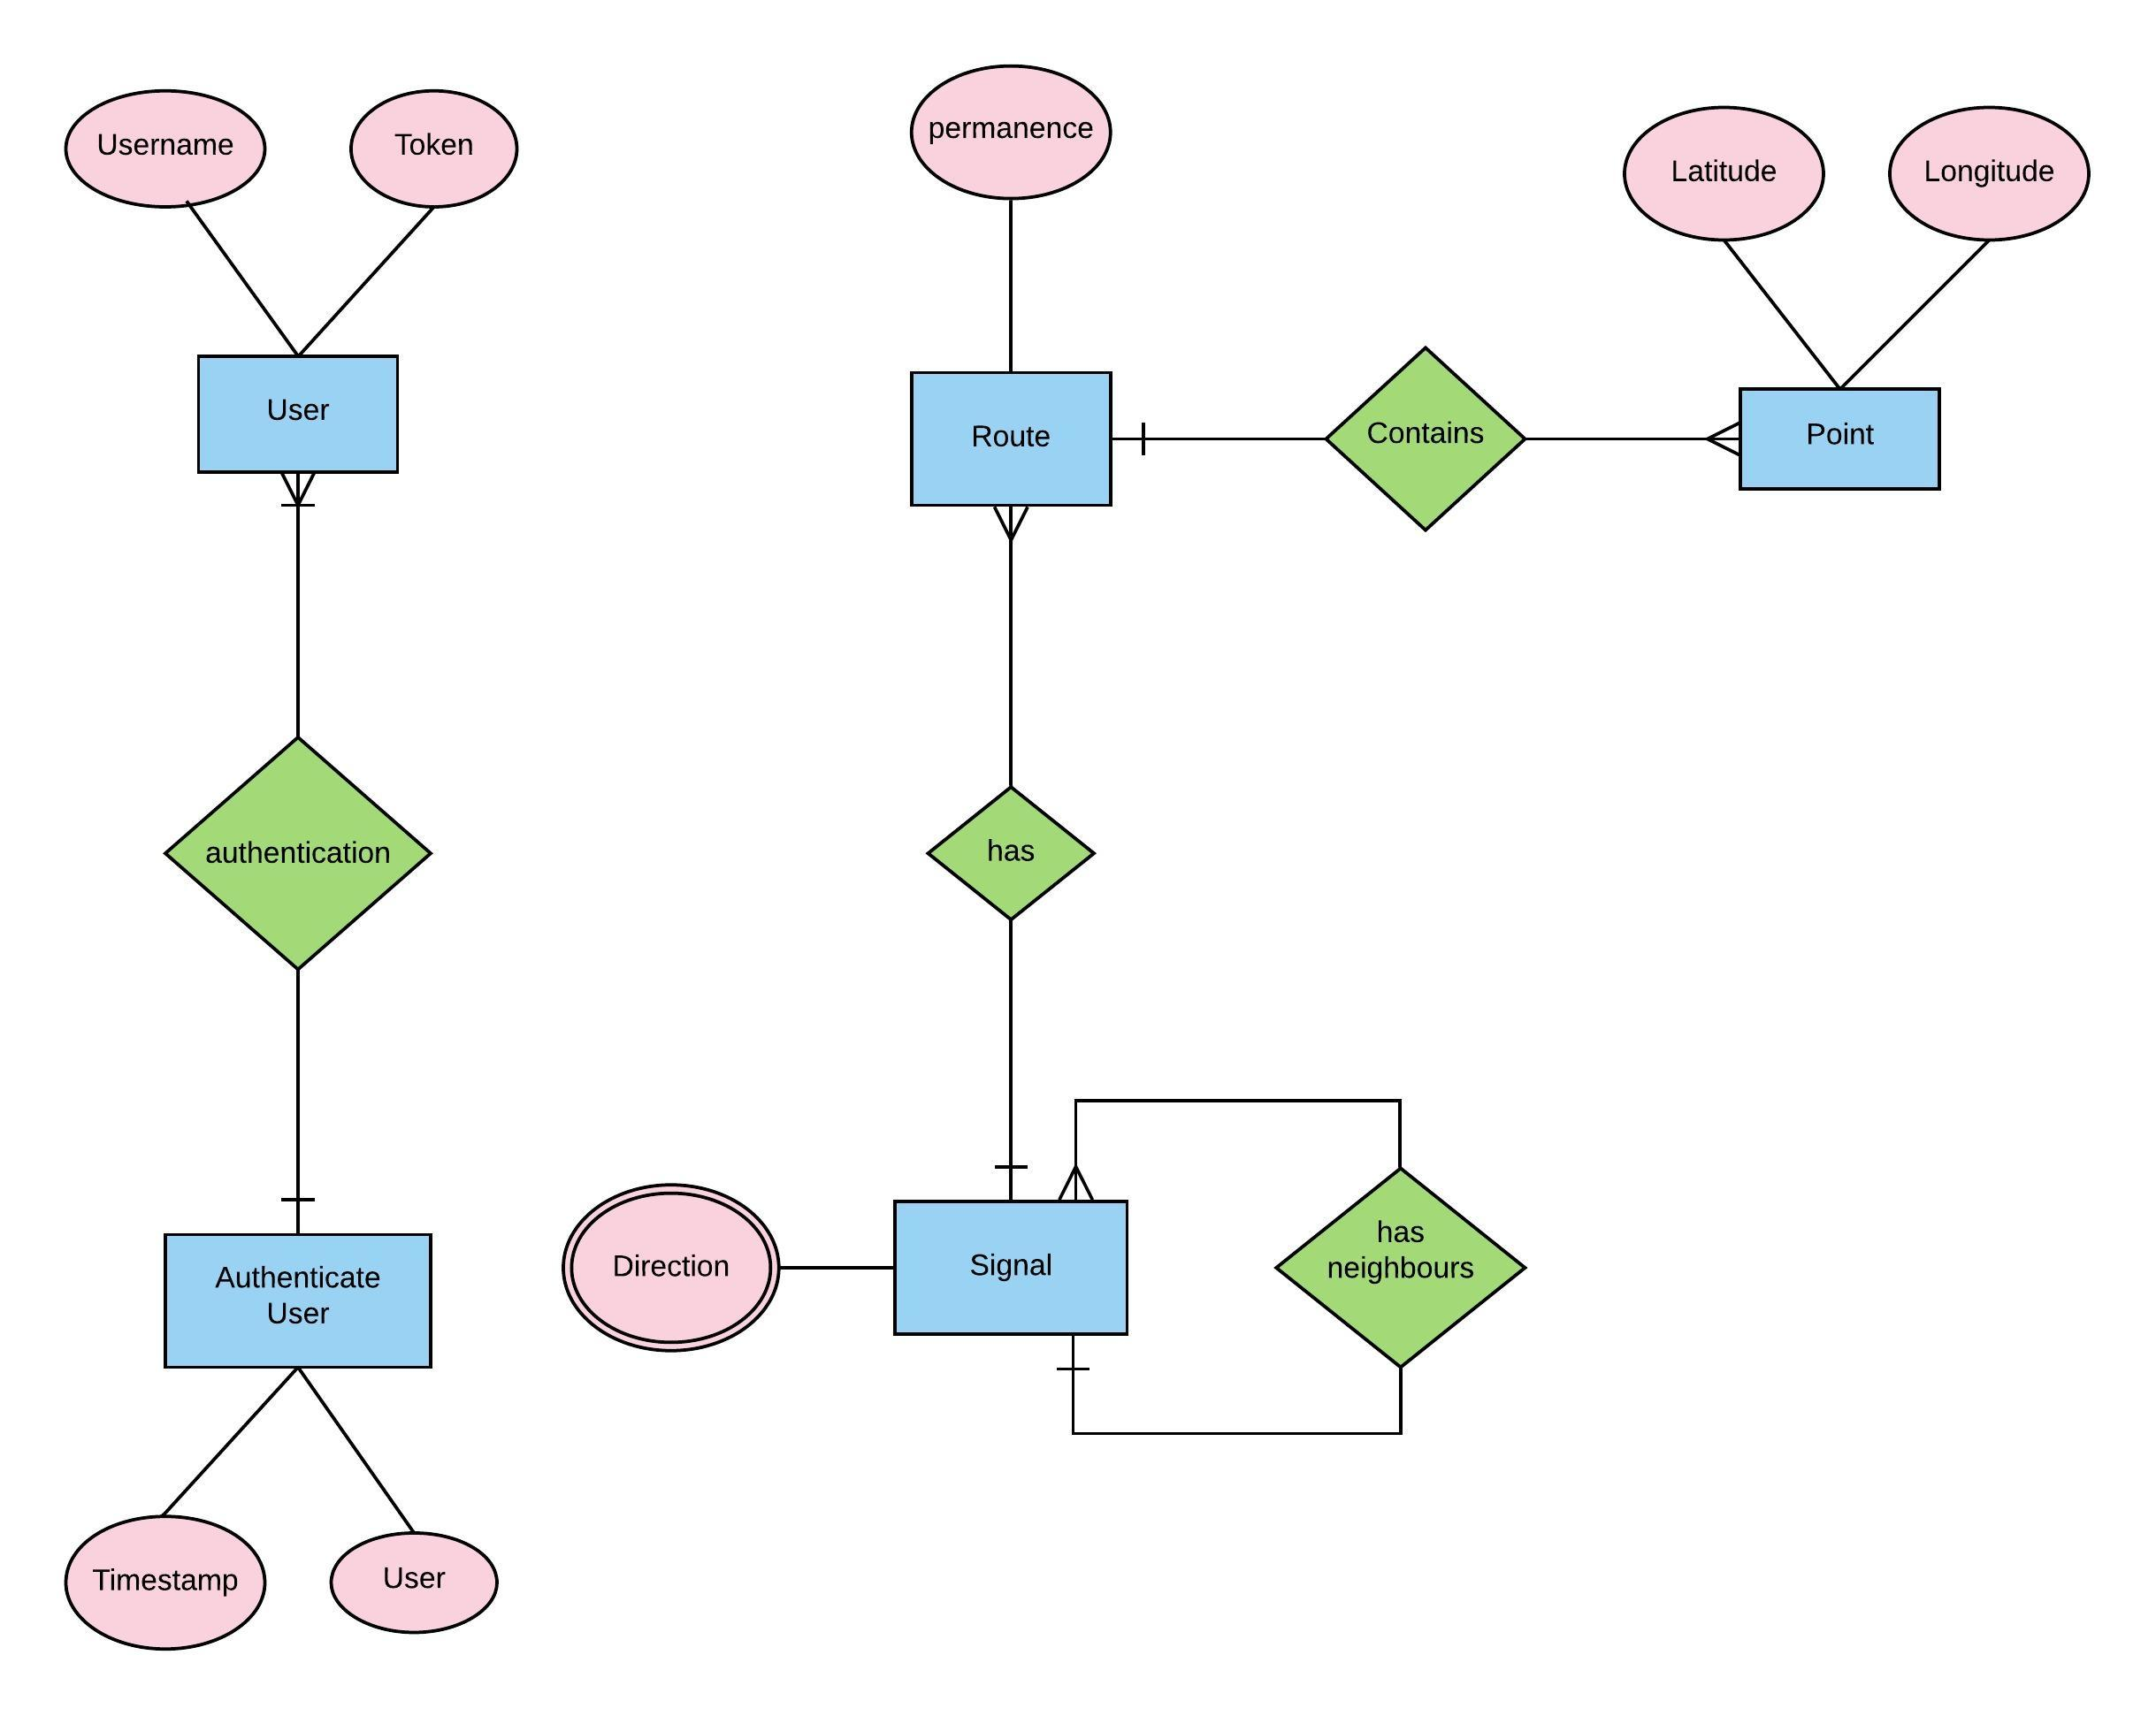
\includegraphics[scale=0.125]{Diagrams/ER_Diagram.jpeg}
		\end{center}
		\caption{ER Diagram}
	\end{figure}


\chapter{Coding}

\section{Algorithms / Flowcharts}
\section{Software used}
\begin{itemize}
    \item MOTUS tool (Mircroscopic Open Traffic Simulator)
    \item Redis Database
    \item python-json
    \item Django web server (modified)
    \item GoogleMaps web API
\end{itemize}

\section{Hardware specification}
\begin{itemize}
    \item LoRa comms wireless card.
    \item Atmega or ESP microprocessor board.
\end{itemize}

\section{Programming language}
\begin{itemize}
    \item JavaScript
    \item HTML+CSS
    \item Embedded C / Python (test phase)
\end{itemize}

\section{Platform}
\begin{itemize}
    \item Atmega/ESP/STM32 core microcontroller.
    \item Google Cloud Service.
\end{itemize}

\newpage 


\section{Components}

%in case we make a mistake, rather discuss
\section{Tools}
\begin{itemize}
    \item Arduino IDE
    \item Git (hosted over Github)
    \item LEMP stack (Linux + Nginx + MySQL + Python)
\end{itemize}


\chapter{Results}


\chapter{Testing}
\section{Formal technical reviews} %?????????????? le fugg
\section{Test plan}
\section{Test cases}
\section{Test Results}
(Unit, integration, regression, system, alpha, Beta)


\chapter{Deployment and Maintenance}

     
\chapter{Conclusion and Future Scope}
Write  summary , conclusion in 50 words and future scope
 
%\renewcommand{\appendixname}{Annexure}
%\renewcommand{\bibname}{References}

\addcontentsline{toc}{chapter}{References}
\chapter*{References}
- Follow the format strictly.
%\bibliography{References}



%\renewcommand{\chaptername}{References}
%\begin{thebibliography}{999}
%\addcontentsline{toc}{chapter}{\numberline{}References}
%\end{thebibliography}



\begin{appendices}


%\chapter{References}
%(Strictly in ACM Format)

% \chapter{ALGORITHMIC DESIGN}
\chapter{Laboratory assignments from Term I}


\chapter{Laboratory assignments on Project Quality and Reliability Testing of Project Design}

It should include assignments such as
\begin{itemize}
\item Use of divide and conquer strategies to exploit distributed/parallel/concurrent processing of the above to identify object, morphisms, overloading in functions (if any), and functional relations and any other dependencies (as per requirements).
             It can include Venn diagram, state diagram, function relations, i/o relations; use this to derive objects, morphism, overloading

\item Use of above to draw functional dependency graphs and relevant Software modeling methods, techniques
including UML diagrams or other necessities using appropriate tools.
\item Testing of project problem statement using generated test data (using mathematical models, GUI, Function testing principles, if any) selection and appropriate use of testing tools, testing of UML diagram's reliability. Write also test cases [Black box testing] for each identified functions. 
You can use Mathematica or equivalent open source tool for generating test data. 
\item Additional assignments by the guide. If project type as Entreprenaur, Refer \cite{ehr},\cite{mckinsey},\cite{mckinseyweb}, \cite{govwebsite}
\end{itemize}







\chapter{Reviewers Comments of Paper Submitted}
(At-least one technical paper must be submitted in Term-I on the project design in the
conferences/workshops in IITs, Central Universities or UoP Conferences or equivalent International Conferences Sponsored by IEEE/ACM)
\begin{enumerate}
\item Paper Title:
\item Name of the Conference/Journal where paper submitted :
\item Paper accepted/rejected : 
\item Review comments by reviewer :
\item Corrective actions if any :  

\end{enumerate}

\chapter{Plagiarism Report}
Plagiarism report
\chapter{ Term-II Project Laboratory Assignments}
\begin{enumerate}
\item Review of design and necessary corrective actions taking into consideration the feedback report of Term I assessment, and other competitions/conferences participated like IIT, Central Universities, University Conferences or equivalent centers of excellence etc.
\item Project workstation selection, installations along with setup and installation report preparations.
\item Programming of the project functions, interfaces and GUI (if any) as per 1 st Term term-work submission using corrective actions recommended in Term-I assessment of Term-work.
\item Test tool selection and testing of various test cases for the project performed and generate various testing result charts, graphs etc. including reliability testing.\\
\textbf{Additional assignments for the Entrepreneurship Project:}
\item Installations and Reliability Testing Reports at the client end.

\end{enumerate}
\end{appendices}


\end{document}
